\chapter{Figures}
\label{appendix-figures}


% \section{Burned Area Trends and Correlations}

% \begin{figure}[H]
%     \centering
%     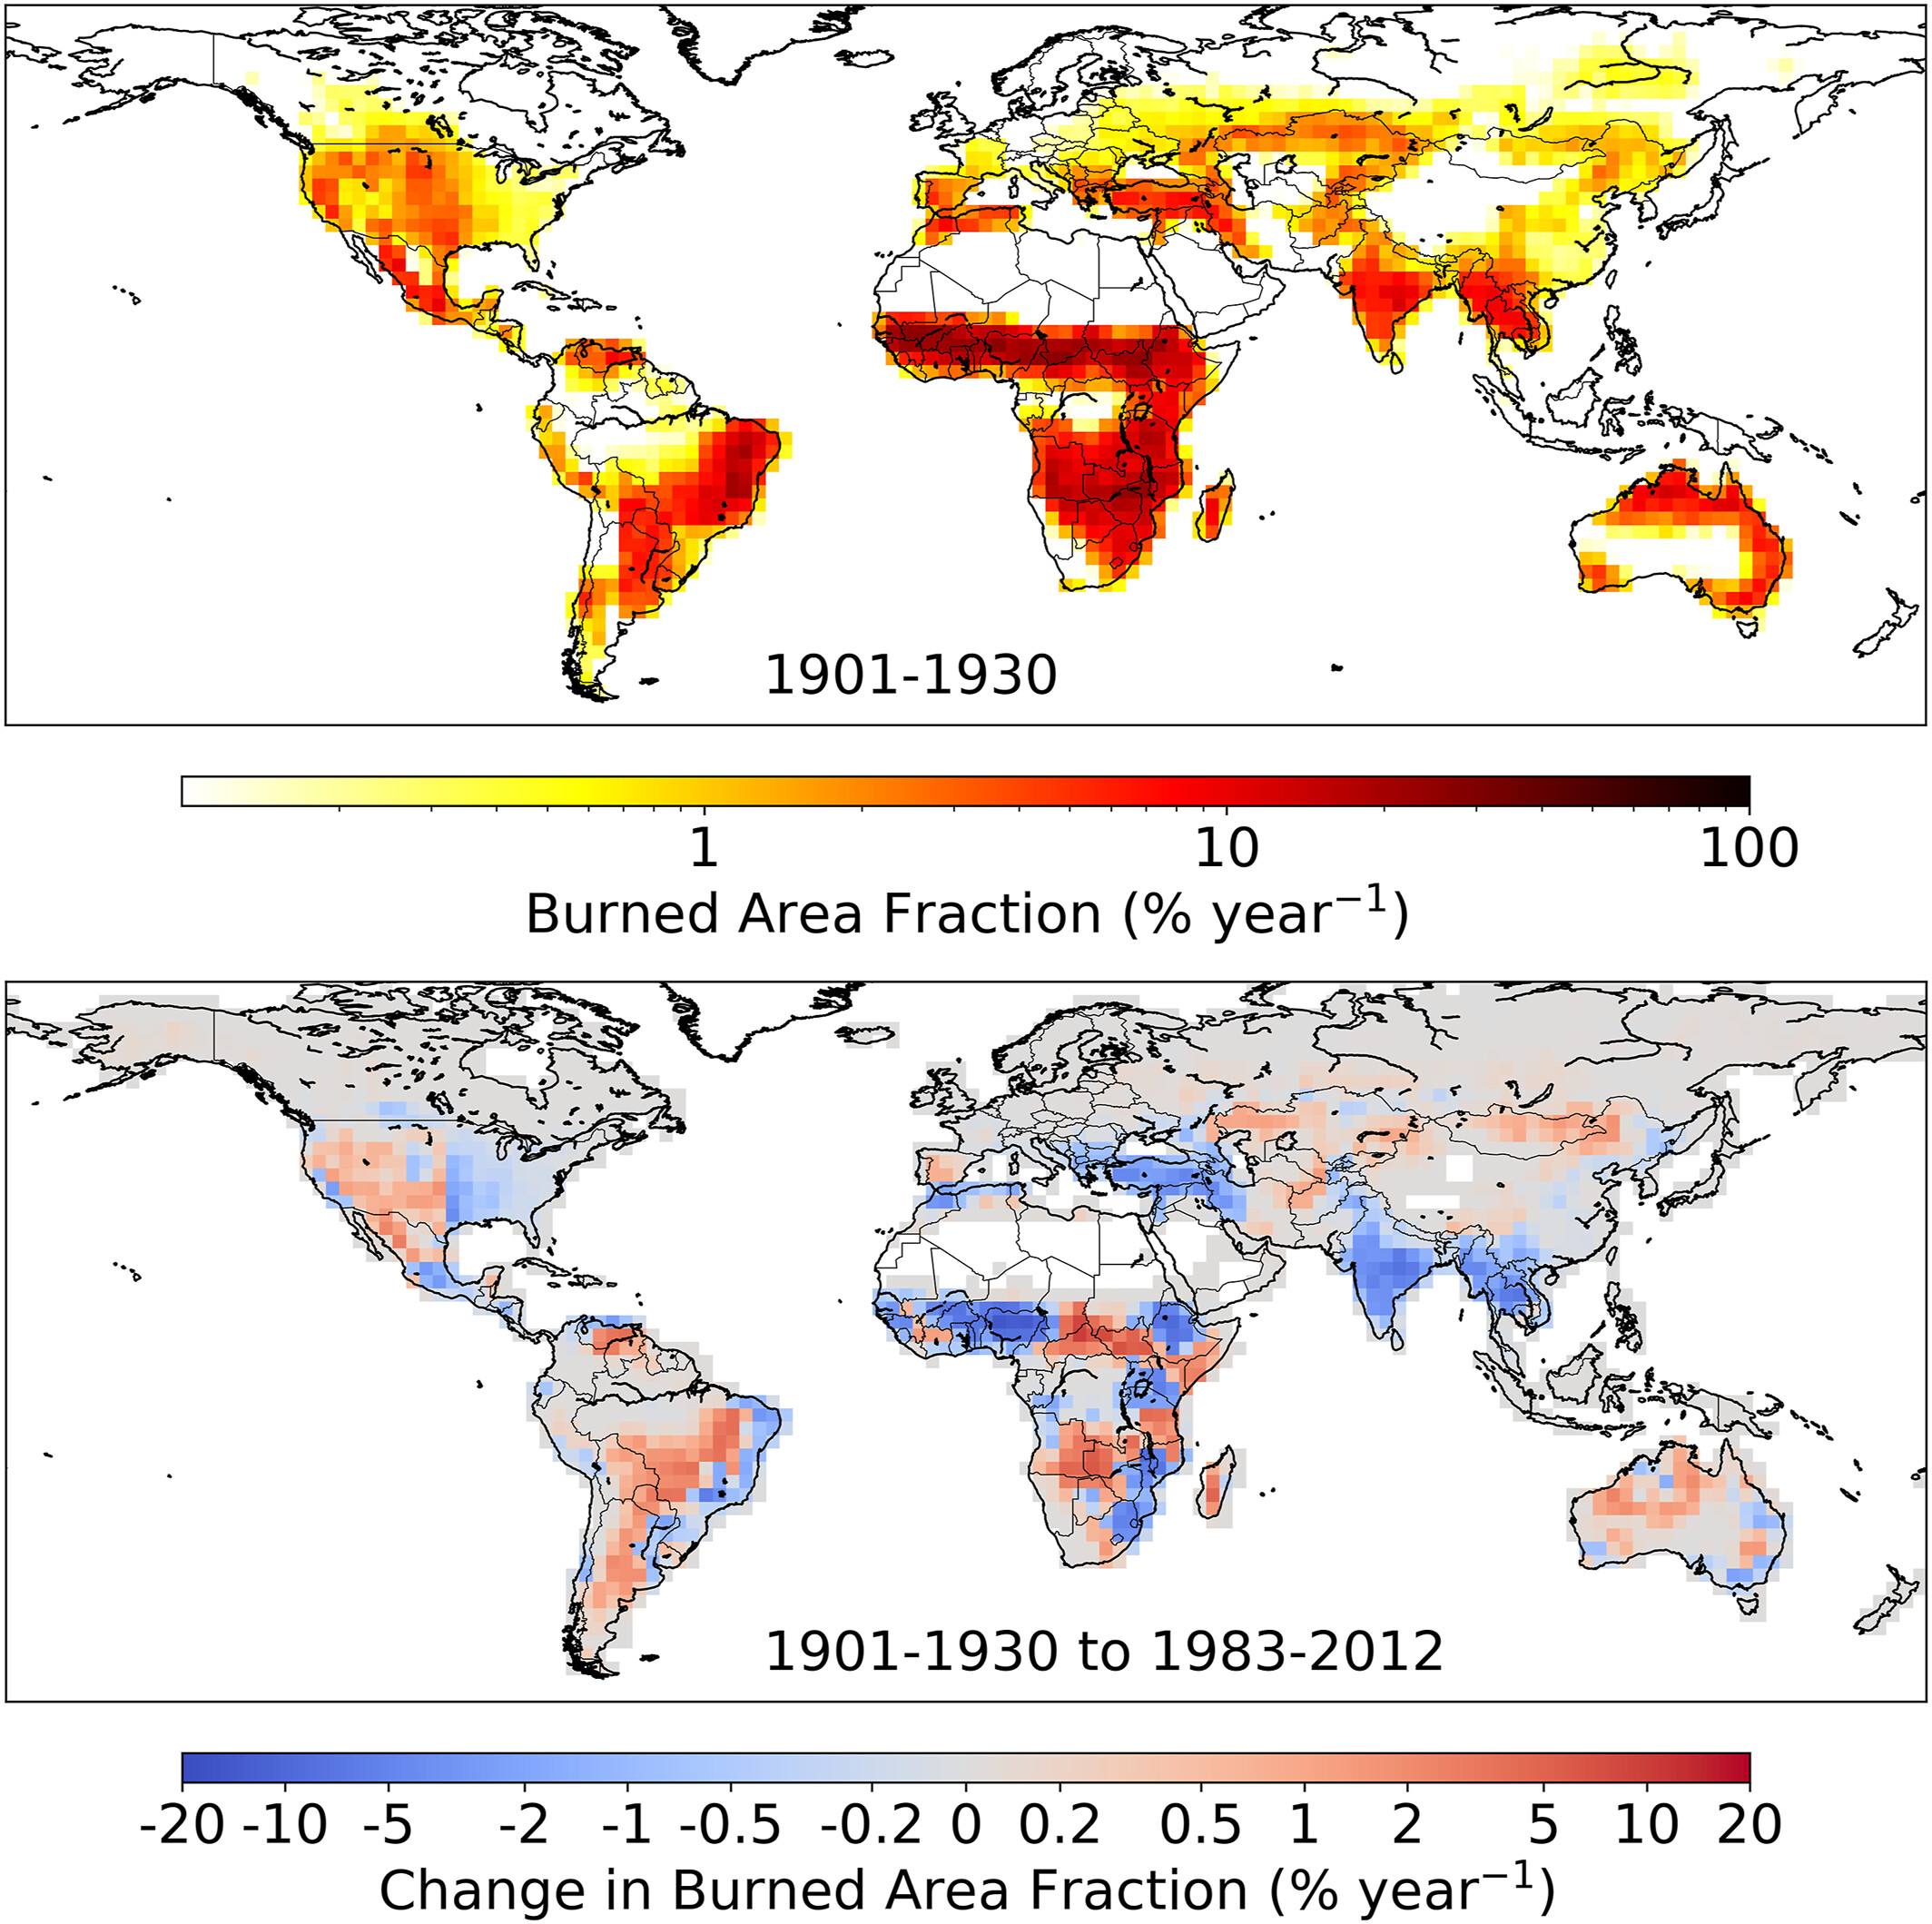
\includegraphics[width=1\linewidth]{images/burned_area_trend_1901_1930.png}
%     \caption{Multi-model median simulations of burned area (BA) fraction during 1901–1930 (\% year−1) and change in BA fraction between the periods 1901–1930 and 1983–2012 (\% year−1) from the ensemble of six Fire Model Intercomparison Project models, gridded at 2.5° resolution. (Top panel) Multi-model median estimate of mean annual BA fraction in the baseline period 1901–1930. (Right panel) Change in the multi-model median estimate of mean annual BA fraction between baseline and modern (1983–2012) periods. The model simulation data derives from Teckentrup et al. ([2019] with updates to two models after Lasslop, Hantson, Harrison, et al.  and Burton et al. ([2019]; see Text A in Supporting Information [S1].}
%     \label{fig:BA_trend_}
% \end{figure}

% \begin{figure}
%     \centering
%     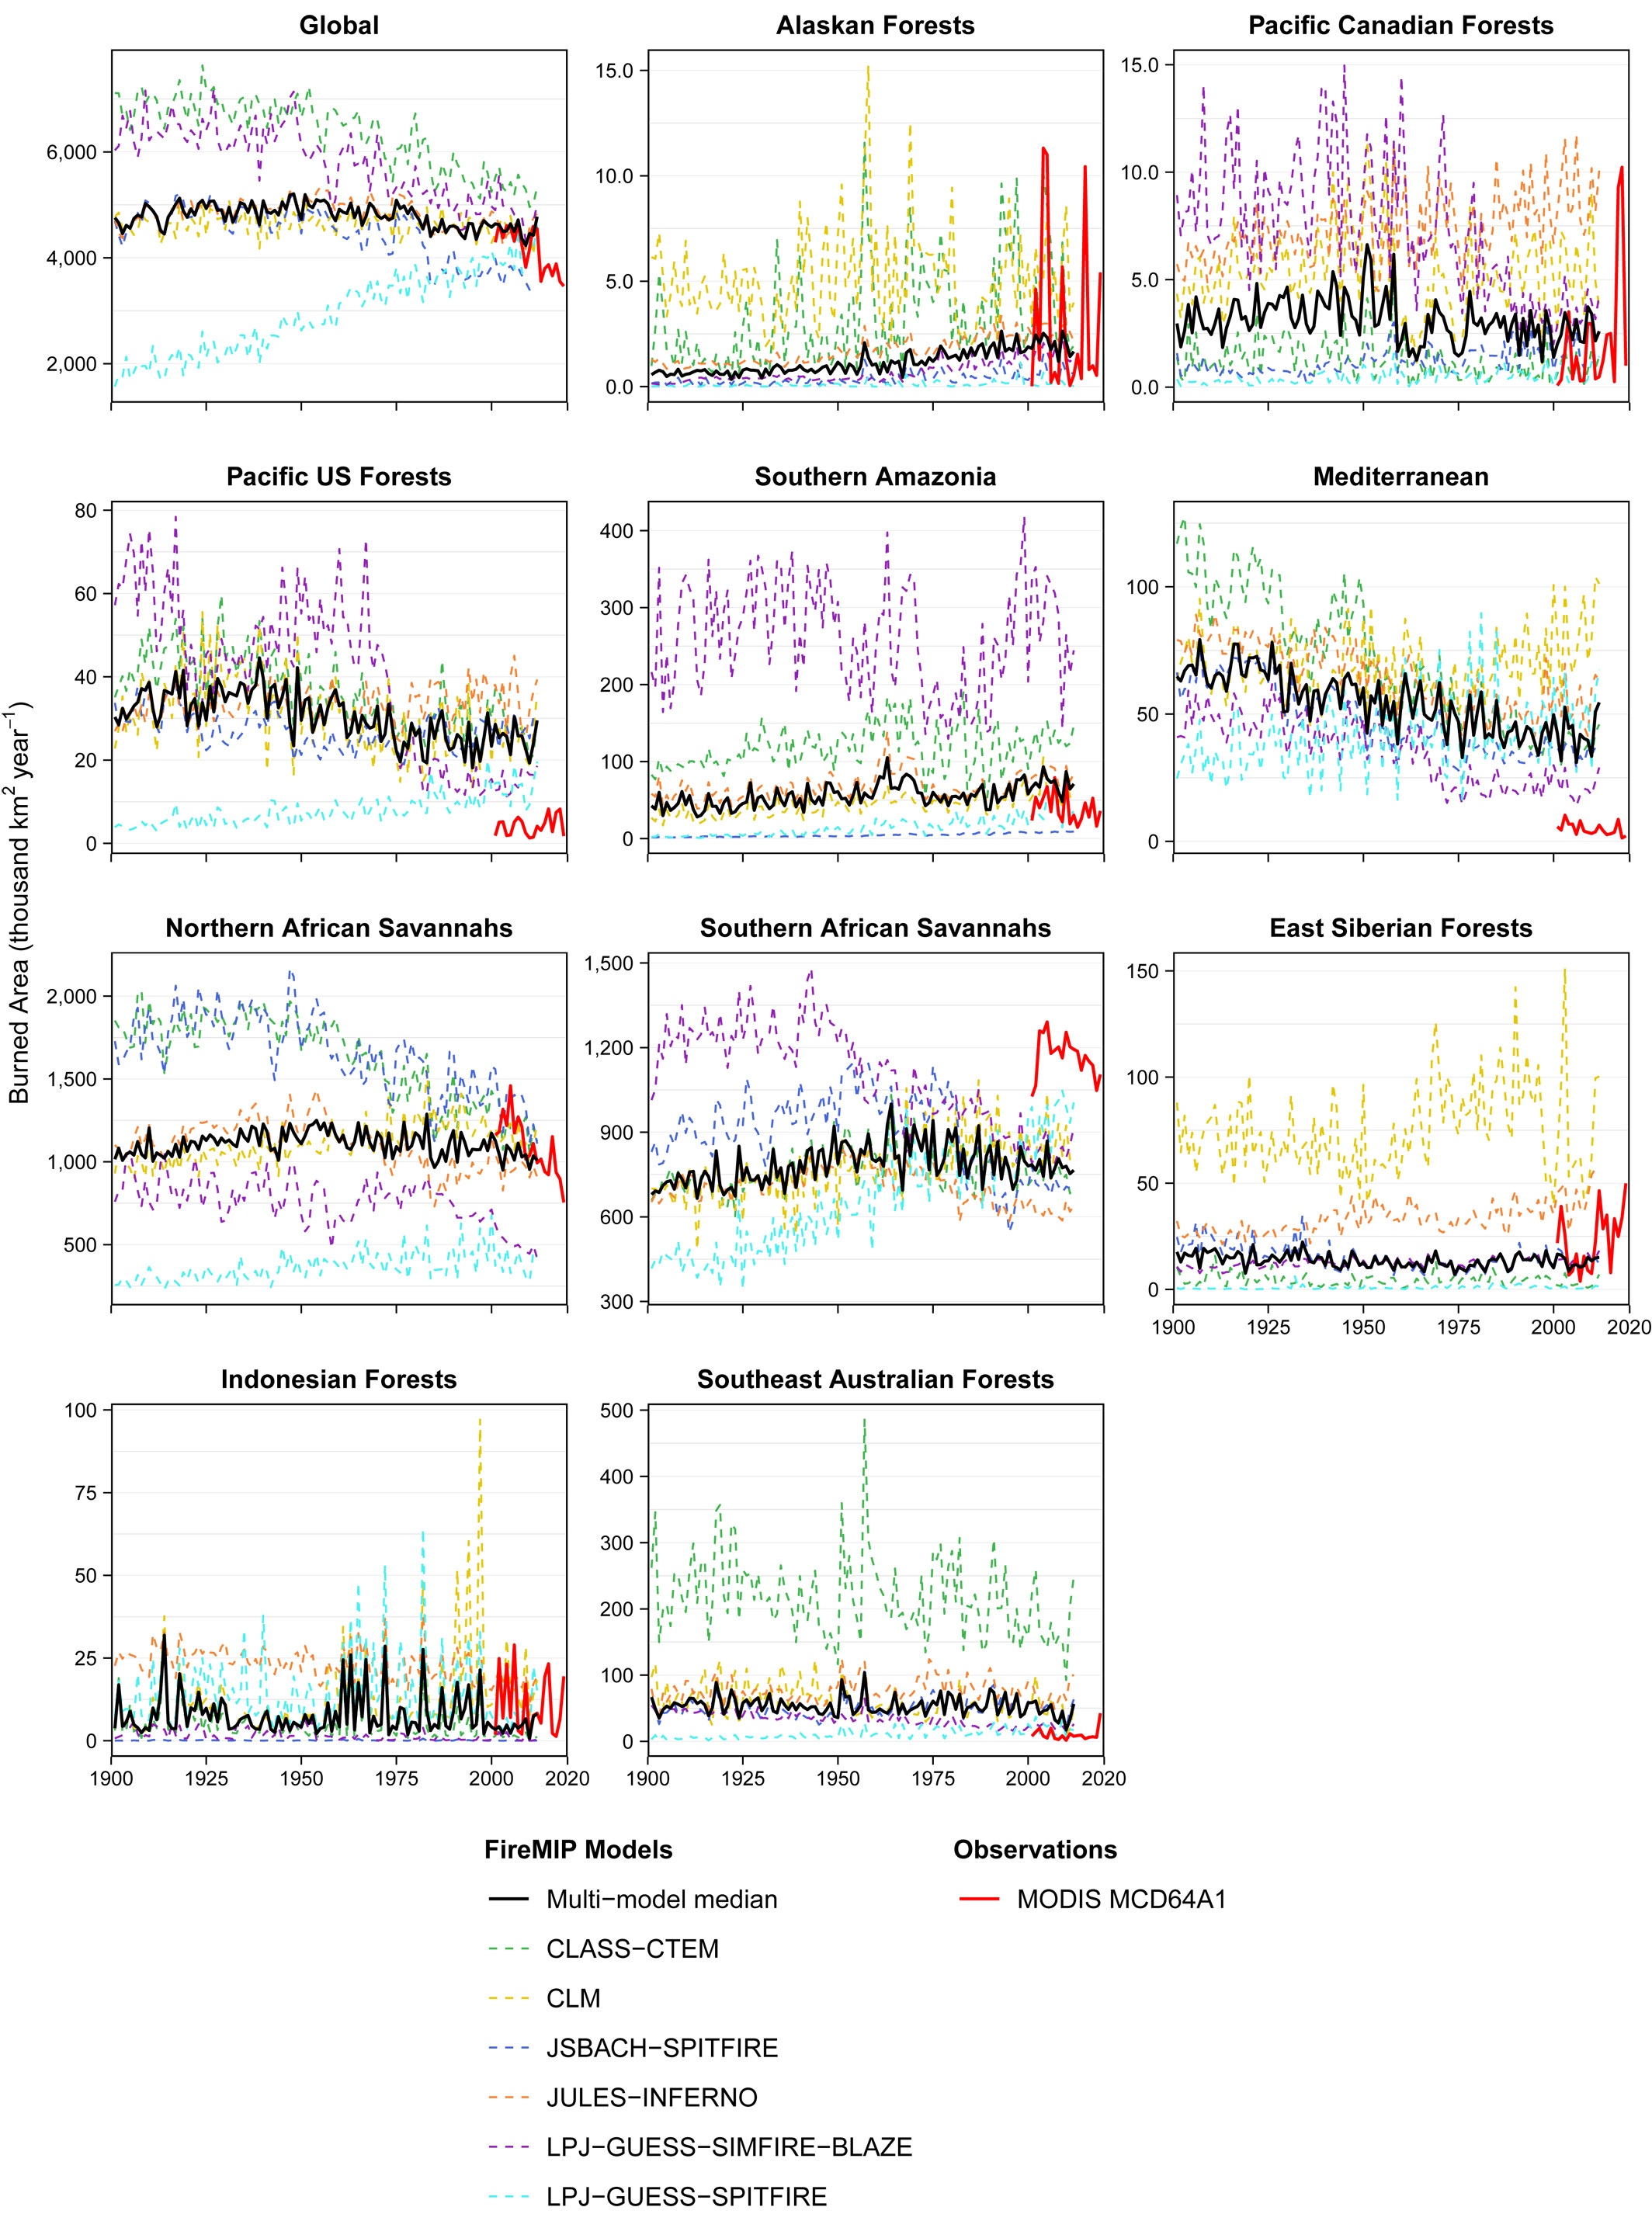
\includegraphics[width=0.8\linewidth]{images/regional_series_fireMip.png}
%     \caption{Regional time series of global and regional burned area (BA) modeled by six fire-enabled dynamic global vegetation models run offline as part of Fire Model Intercomparison Project (FireMIP) (dashed lines for individual models) (Teckentrup et al., \href{https://agupubs.onlinelibrary.wiley.com/doi/full/10.1029/2020RG000726\#rog20279-bib-0513}{2019}). The solid black lines plot the multi-model median annual BA from the FireMIP models. The solid red lines (2001–2019) plot observed BA from the moderate resolution imaging spectroradiometer BA product (Giglio et al., \href{https://agupubs.onlinelibrary.wiley.com/doi/full/10.1029/2020RG000726\#rog20279-bib-0201}{2018}). The model simulation data derives from Teckentrup et al. (\href{https://agupubs.onlinelibrary.wiley.com/doi/full/10.1029/2020RG000726\#rog20279-bib-0513}{2019}) with updates to two models after Lasslop, Hantson, Harrison, et al. (\href{https://agupubs.onlinelibrary.wiley.com/doi/full/10.1029/2020RG000726\#rog20279-bib-0309}{2020}) and Burton et al. (\href{https://agupubs.onlinelibrary.wiley.com/doi/full/10.1029/2020RG000726\#rog20279-bib-0081}{2019}; see Text A in Supporting Information \href{https://agupubs.onlinelibrary.wiley.com/doi/full/10.1029/2020RG000726\#support-information-section}{S1} for methods). }
%     \label{fig:regional_series_fireMip}
% \end{figure}

% burned Area Current trend

% \begin{figure}[H]
%     \centering
%     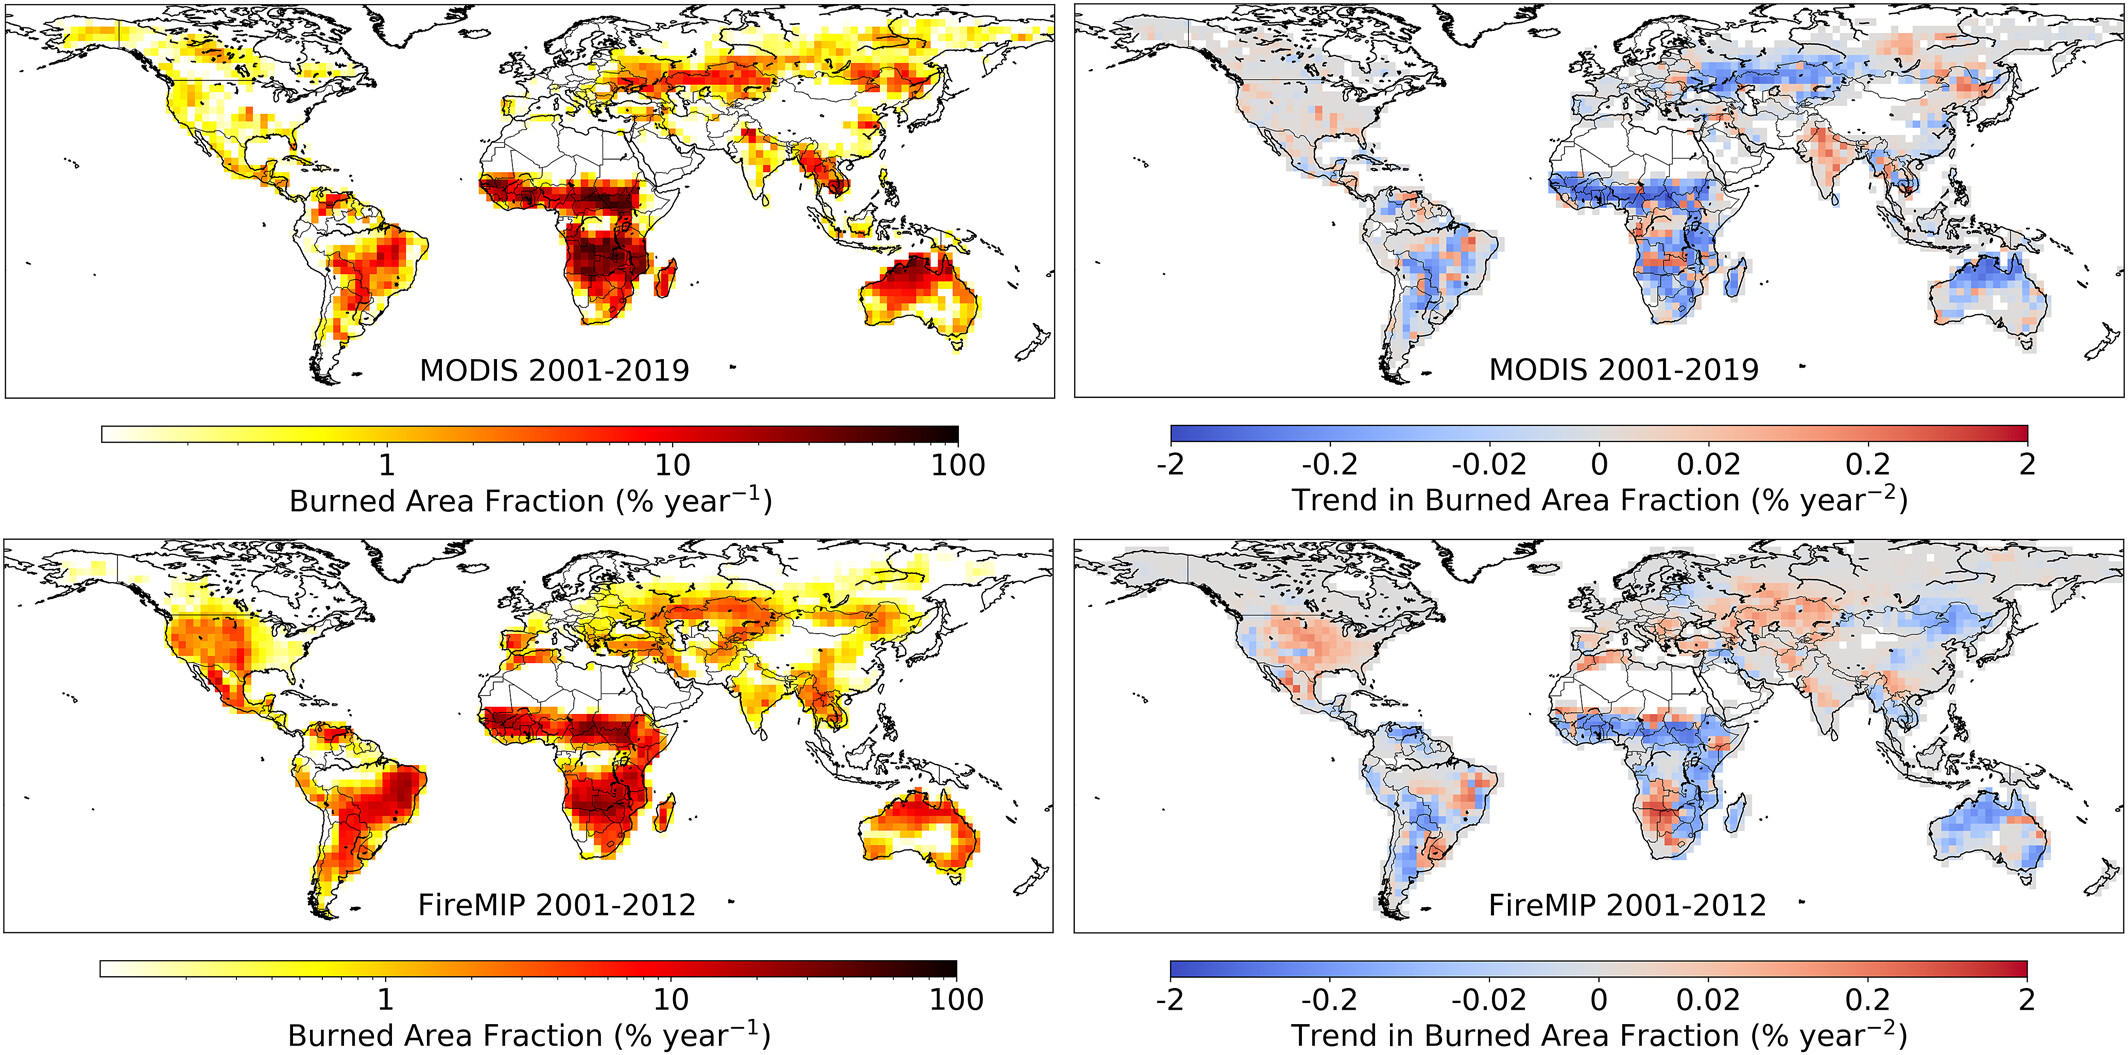
\includegraphics[width=1\linewidth]{images/BA_trend_2001_2019.png}
%     \caption{Global observed and modeled burned area (BA) fraction and their trends during the periods shown, gridded at 2.5° resolution (Giglio et al., [2018]; Teckentrup et al., [2019]. Plots show (left panels) annual mean BA fraction (\% year−1) and (right panels) trend in BA fraction (\% year−2) since 2001 period for (upper panels) moderate resolution imaging spectroradiometer BA (2001–2019) and (lower panels) six Fire Model Intercomparison Project (FireMIP) models (2001–2012). Year 2012 is the final year for which FireMIP simulations are available. The slope is calculated as the Theil-Sen estimator, which is insensitive to outliers.}
%     \label{fig:BA_trend_2001_2019}
% \end{figure}

% \begin{figure}[H]
%     \centering
%     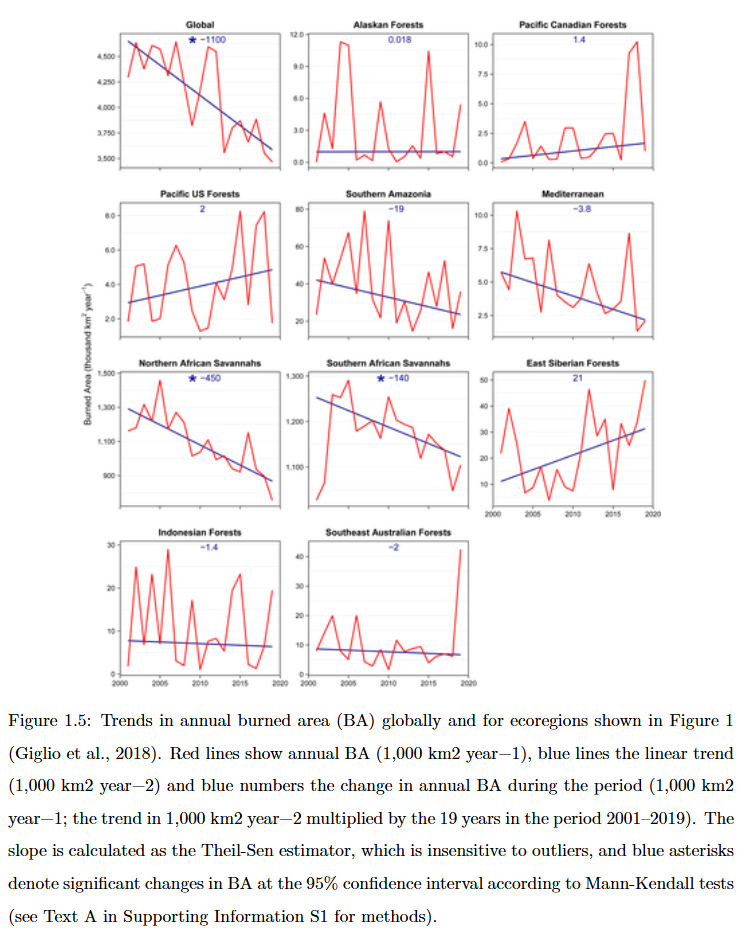
\includegraphics[width=1\linewidth]{images/BA_global_trend_regions.png}
%     \caption{Enter Caption}
%     \label{fig:BA_global_trend_regions}
% \end{figure}

% \begin{figure}[H]
%     \centering
%     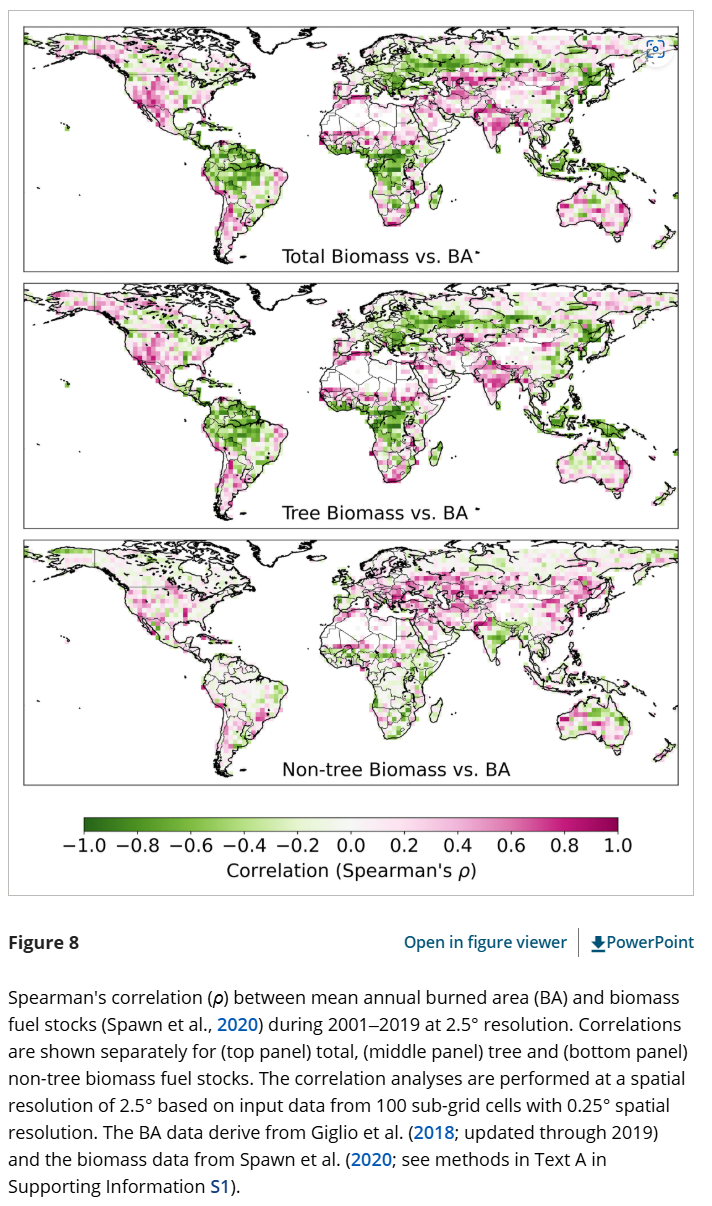
\includegraphics[width=1\linewidth]{images/map_BA_correlation_biomass_BA.png}
%     \caption{Enter Caption}
%     \label{fig:app_map_BA_correlation_biomass_BA}
% \end{figure}

% \begin{figure}[H]
%     \centering
%     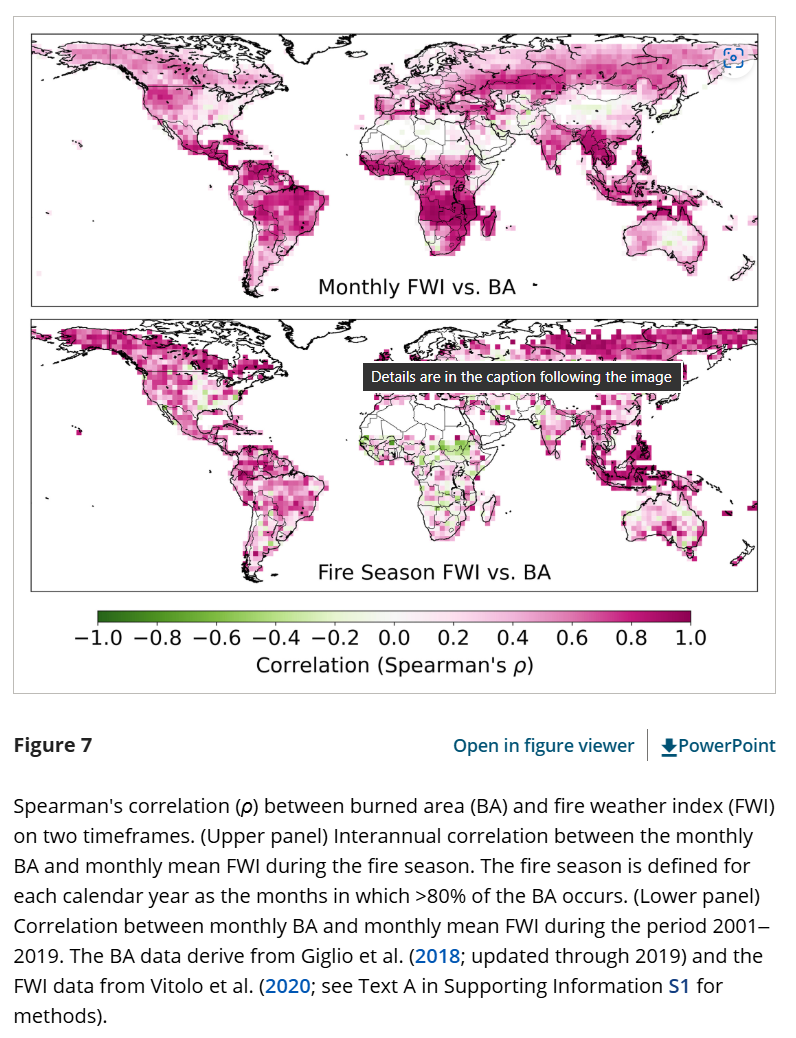
\includegraphics[width=1\linewidth]{images/map_BA_correlation_FWI.png}
%     \caption{Enter Caption}
%     \label{fig:app_map_BA_correlation_FWI}
% \end{figure}

% \begin{figure}[H]
%     \centering
%     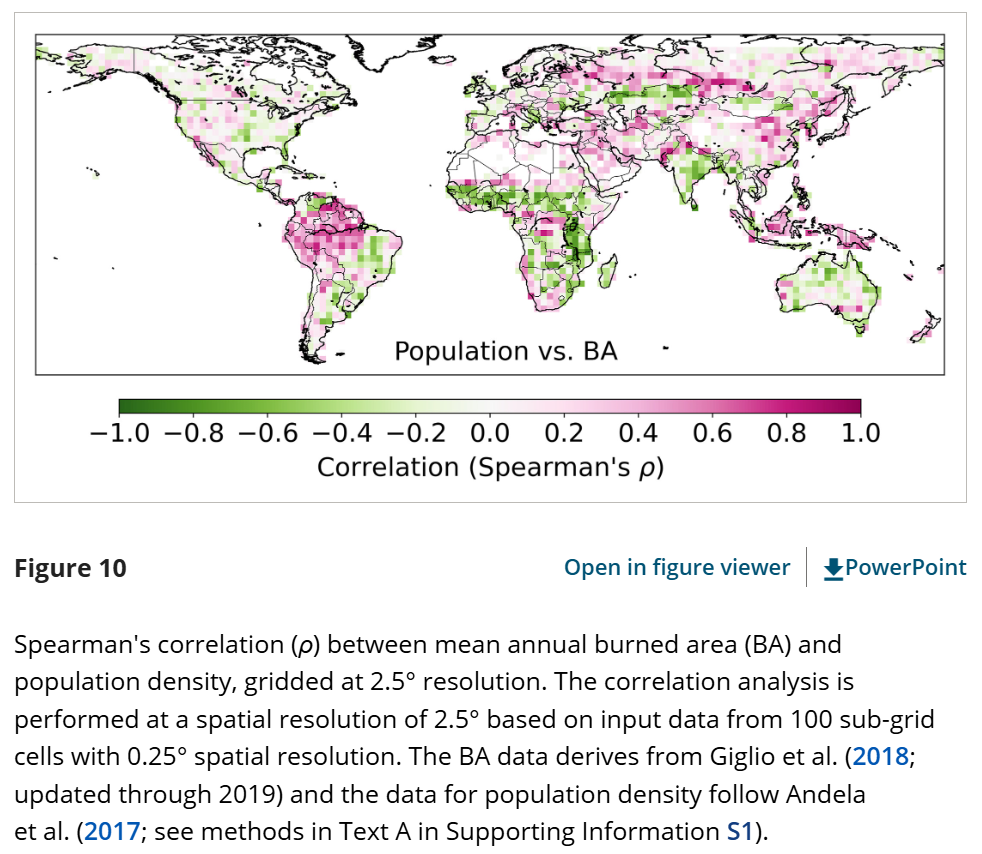
\includegraphics[width=1\linewidth]{images/map_BA_correlation_population.png}
%     \caption{Enter Caption}
%     \label{fig:app_map_BA_correlation_population}
% \end{figure}


%%% ================================================================
%%% Fire Season Maps (moved from Chapter~2)
%%% ================================================================
\section{Fire Season Maps}
\label{sec:appendix_fire_season_maps}

\begin{figure}[H]
    \centering
    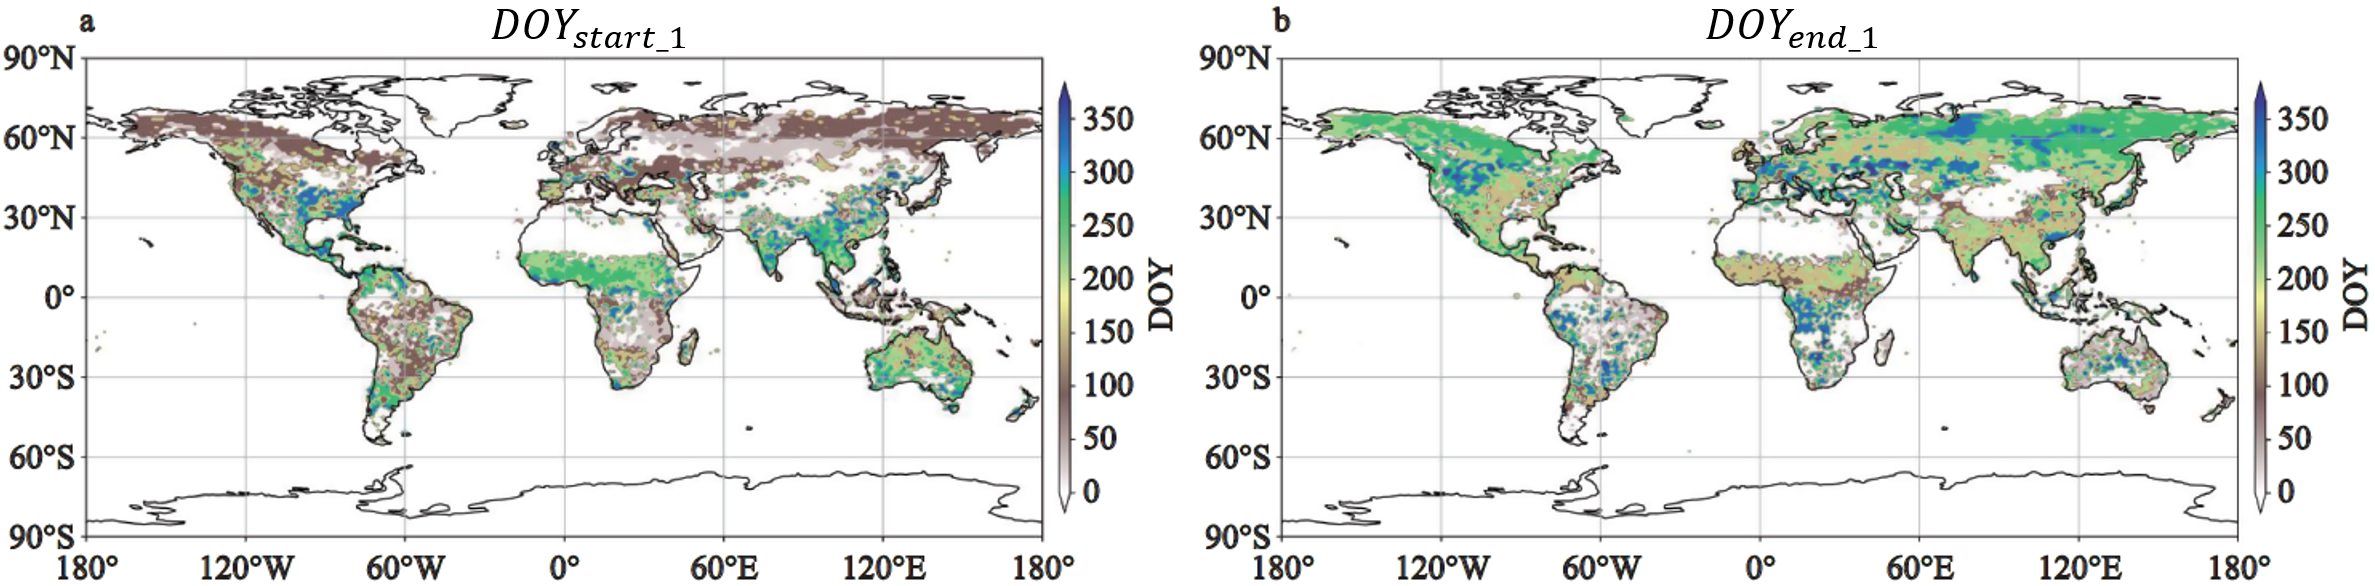
\includegraphics[width=0.9\linewidth]{images/fire_season_start1_end1.png}
    \caption{\footnotesize{Global distributions of the fire season first subperiod (see Fig. \ref{fig:fire_season_types})  start day of year $\mathrm{DOY}_{\text{start 1}}$  (a) and end $\mathrm{DOY}_{\text{end 1}}$ (b).  \textsuperscript{\ref{fn:Zhang2025}}}}
    \label{fig:fire_season_start_end}
\end{figure}

\begin{figure}[H]
    \centering
    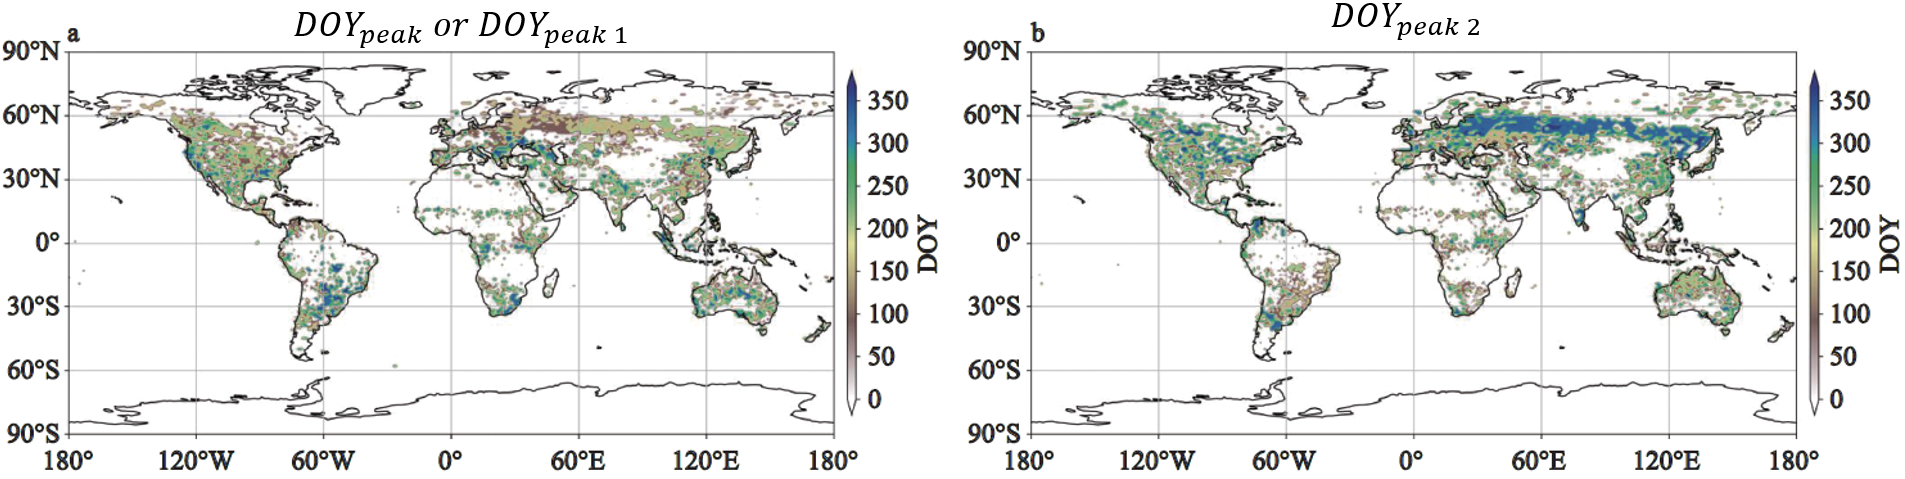
\includegraphics[width=1\linewidth]{images/fire_season_peaks.png}
    \caption{\footnotesize{Global distributions of the peak start day of year $\mathrm{DOY}_{\text{peak} 1}$ in the first subperiod (a) and second subperiod $\mathrm{DOY}_{\text{peak}  2}$(b) of fire season from 2001 to 2022. See Fig.~\ref{fig:fire_season_types} for subperiod definitions.  \textsuperscript{\ref{fn:Zhang2025}}}}
    \label{fig:fire_season_peaks}
\end{figure}

\begin{figure}[H]
    \centering
    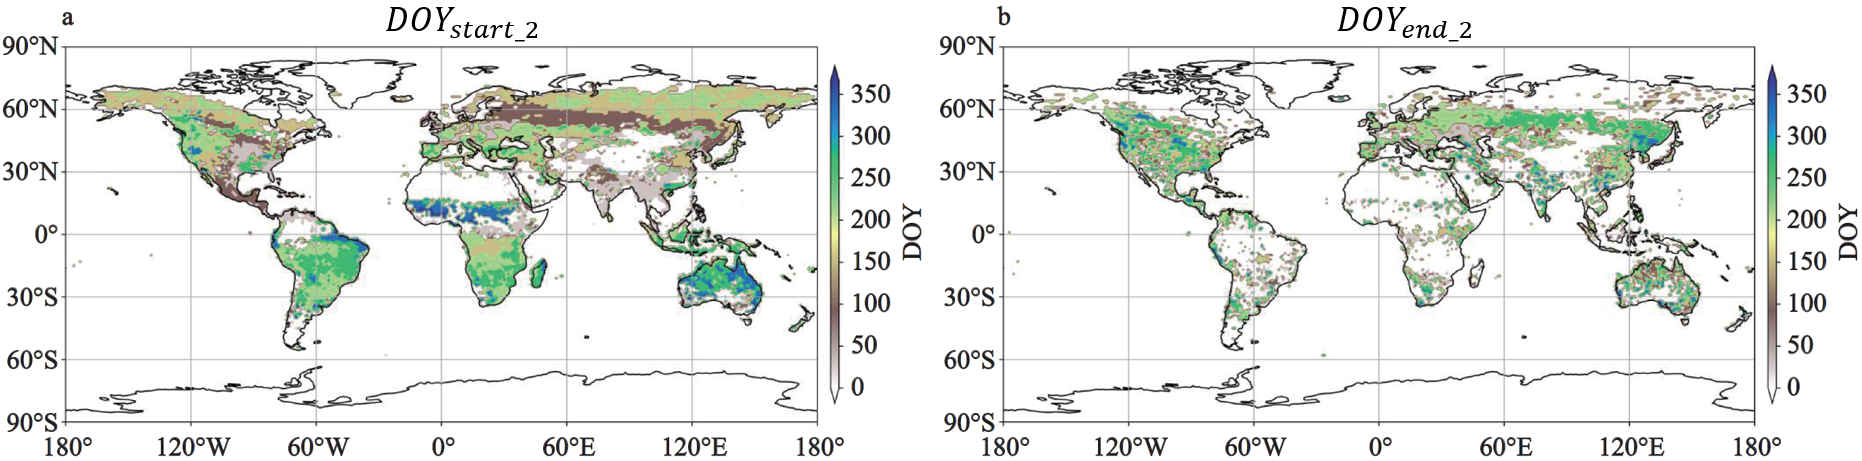
\includegraphics[width=1\linewidth]{images/fire_season_start2_end2.png}
    \caption{\footnotesize{Global distributions of the fire season second subperiod start day of year $\mathrm{DOY}_{\text{start 2}}$ (a) and end $\mathrm{DOY}_{\text{end 2}}$ (b); see Fig.~\ref{fig:fire_season_types} for subperiod definitions.  \textsuperscript{\ref{fn:Zhang2025}}}}
    \label{fig:fire_season_start2_end2}
\end{figure}


%%% ================================================================
%%% Baseline FPR Coverage Maps (moved from Chapter~\ref{chapter-9-the-proposed-system-concept})
%%% ================================================================
\section{$\mathcal{C}_{\text{Zoom}}$ Baseline FPR Coverage Maps ($\eta = 65^{\circ}$)}
\label{sec:appendix_zoom_baseline_fpr}

The following baseline ($\eta = 65^{\circ}$) maps complement the combined recurrent-and-occasional
map retained in Section~\ref{sec:fpr_temporal_coverage_baseline}.

\begin{figure}[H]
    \centering
    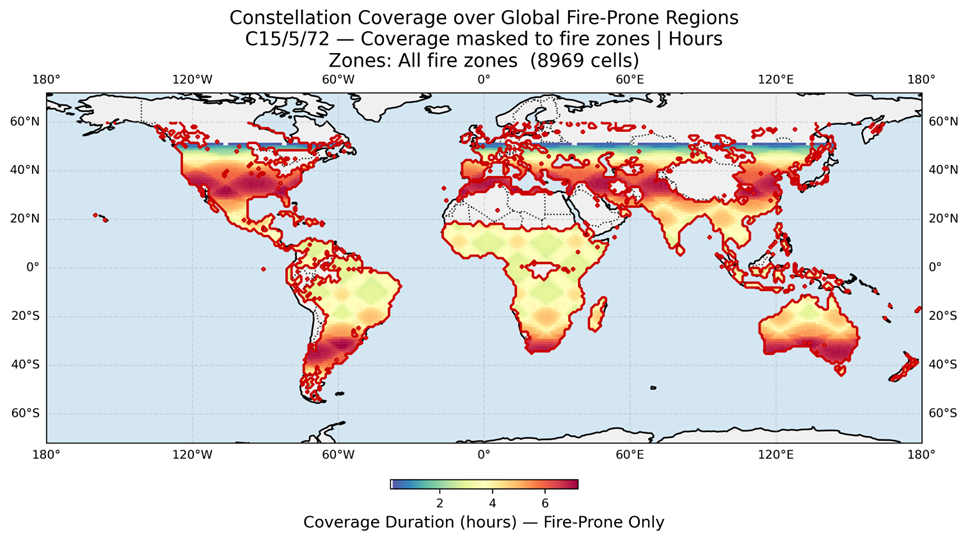
\includegraphics[width=1\linewidth]{images/c_zoom_global_FRP_bondaries_Tcoverage_eta63.png}
    \caption{\footnotesize{Temporal coverage~$T_{\text{cov}}$ of the FPR boundaries mask for $\mathcal{C}_{\text{Zoom}}$ at the baseline $\eta = 65^{\circ}$.  The boundaries mask encompasses all fire-prone cells regardless of recurrence group, showing the full geographic extent monitored by the constellation.}}
    \label{fig:c_zoom_global_FRP_bondaries_Tcoverage_eta63}
\end{figure}

\begin{figure}[H]
    \centering
    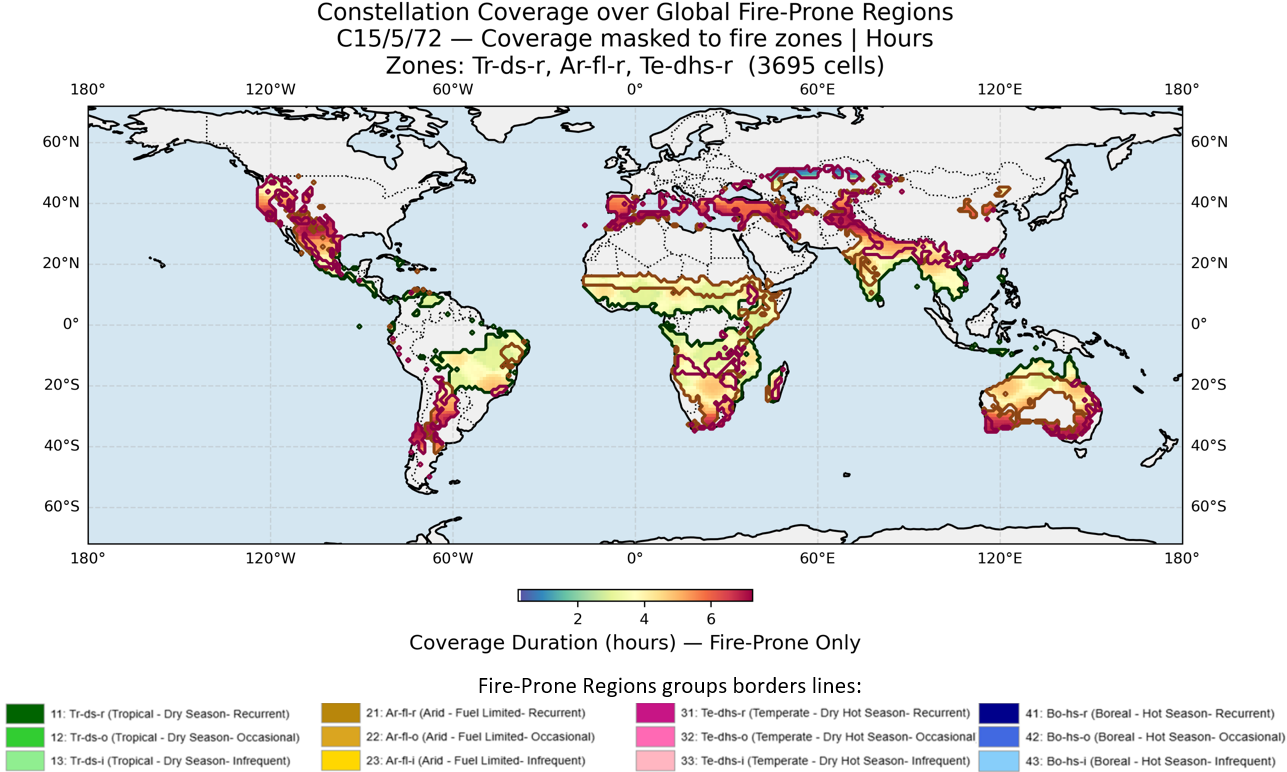
\includegraphics[width=1\linewidth]{images/c_zoom_global_FRP_recurrent_Tcoverage_eta63.png}
    \caption{\footnotesize{Temporal coverage~$T_{\text{cov}}$ of the recurrent-only FPR mask for $\mathcal{C}_{\text{Zoom}}$ at the baseline $\eta = 65^{\circ}$.  Only cells classified as recurrent ($r$, ${>}\,7$~fires/decade) are shown, highlighting the temperate and Mediterranean forest biomes near $\phi \approx \pm\,40^{\circ}$ that constitute the highest-priority monitoring targets.}}
    \label{fig:c_zoom_global_FRP_recurrent_Tcoverage_eta63}
\end{figure}


%%% ================================================================
%%% 7-Day RGTO Seed Propagation Maps (moved from Chapter~8)
%%% ================================================================
\section{7-Day RGTO Seed Propagation Maps}
\label{sec:appendix_7day_maps}

\begin{figure}[H]
    \centering
    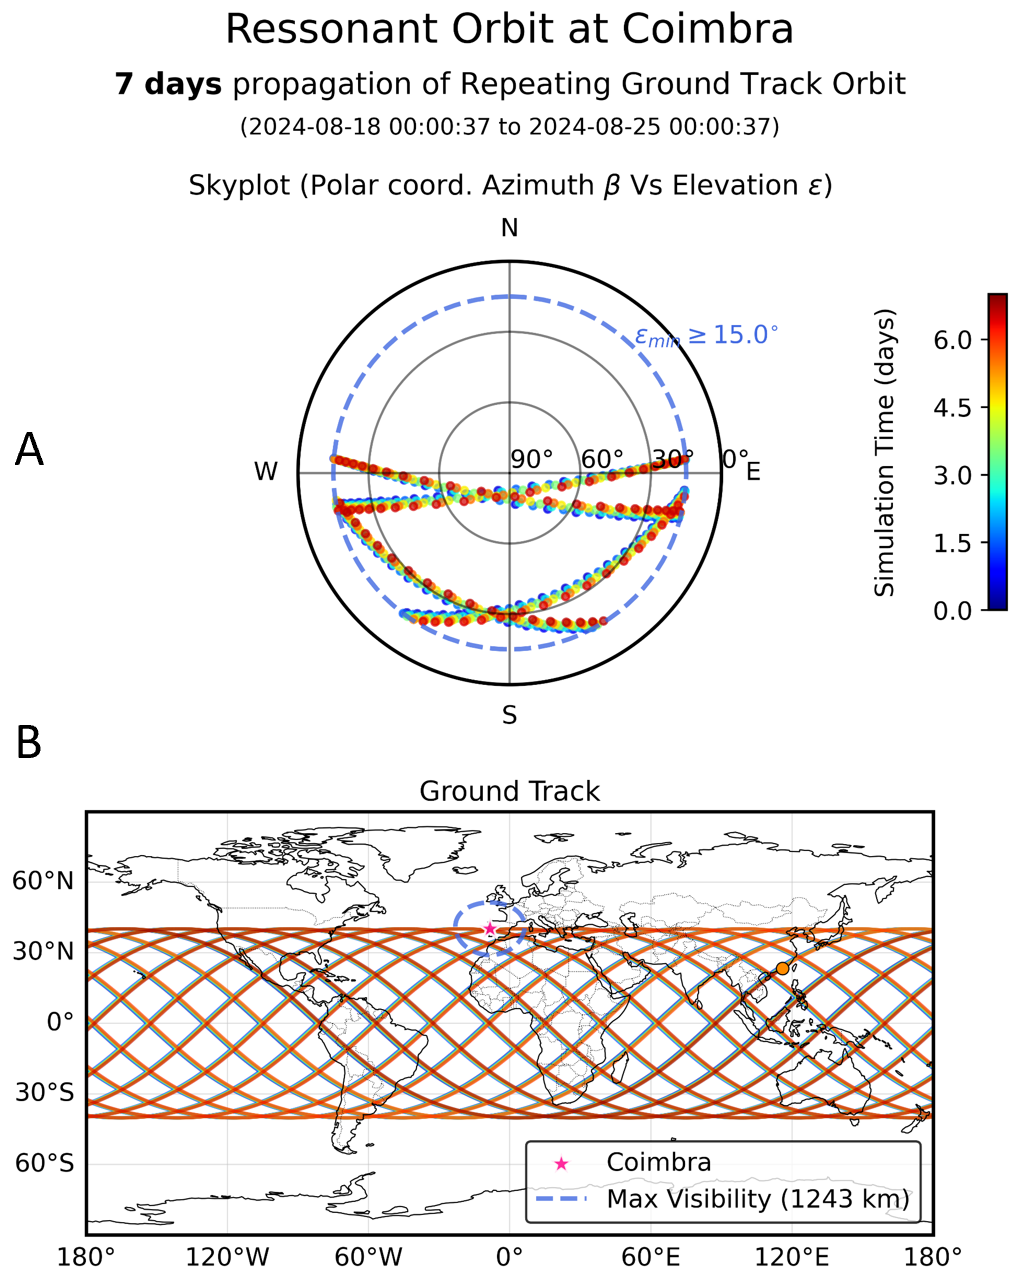
\includegraphics[width=0.8\linewidth]{images/RGTO_maps_Coimbra_Seven_days.png}
    \caption{\footnotesize{7-day RGTO seed propagation over Coimbra without station-keeping ($\tau=15/1$, $h \approx 488$\,km, $i=40.2^{\circ}$).  \textbf{(A)}~Sky plot showing the recurring four-pass cluster with consistent azimuth--elevation trajectories across all seven days.  \textbf{(B)}~Ground track; the trace overlaps the 1-day pattern (Fig.~\ref{fig:RGTO_maps_Coimbra_One_day}), confirming short-term resonance stability under drag and $J_{8\times8}$ perturbations.}}
    \label{fig:RGTO_maps_Coimbra_Seven_days}
\end{figure}


%%% ================================================================
%%% Walker Constellation Example (moved from Chapter~8)
%%% ================================================================
\section{Walker Constellation Illustration}
\label{sec:appendix_walker_example}

\begin{figure}[H]
    \centering
    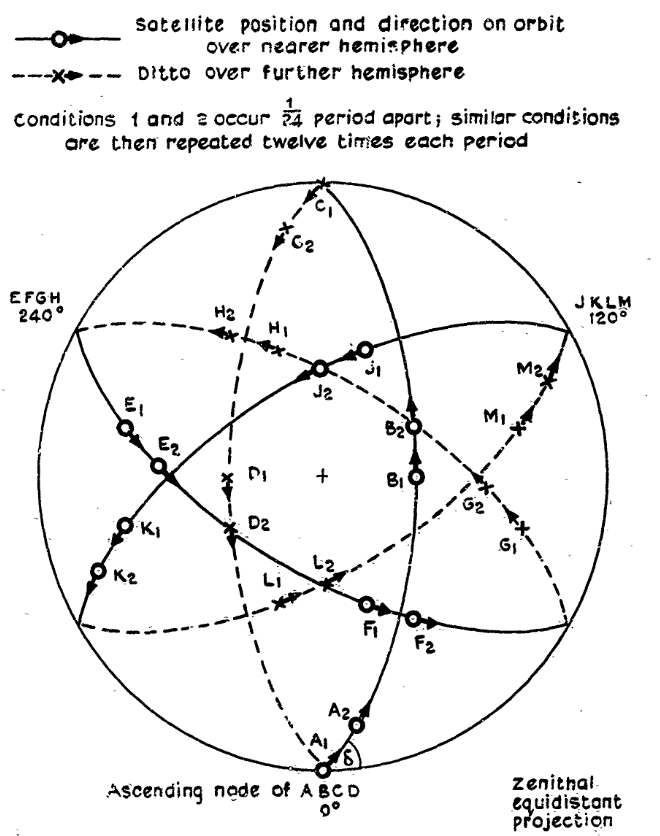
\includegraphics[width=0.4\linewidth]{images/constellation_walker_12_sats_3planes_ example.png}
    \caption{\footnotesize{Walker-$\delta$ constellation example: 12 satellites distributed across 3 orbital planes ($\mathcal{C}_{12/3/120}$), shown in a polar zenithal equidistant projection with the ascending node at the equator as the reference ($\mathrm{RAAN}_{\mathrm{ref}}=0^{\circ}$).  Each plane carries four satellites uniformly phased in true anomaly; the inter-plane RAAN spacing is $120^{\circ}$.  This projection framework is adopted throughout the constellation design \cite{walker_circular_1970}.}}
    \label{fig:constellation_walker_12_sats_3planes_ example}
\end{figure}


%%% ================================================================
%%% 4-Plane Observation Links (moved from Chapter~8)
%%% ================================================================
\section{Four-Plane Constellation Observation Links}
\label{sec:appendix_4plane_obs}

\begin{figure}[H]
    \centering
    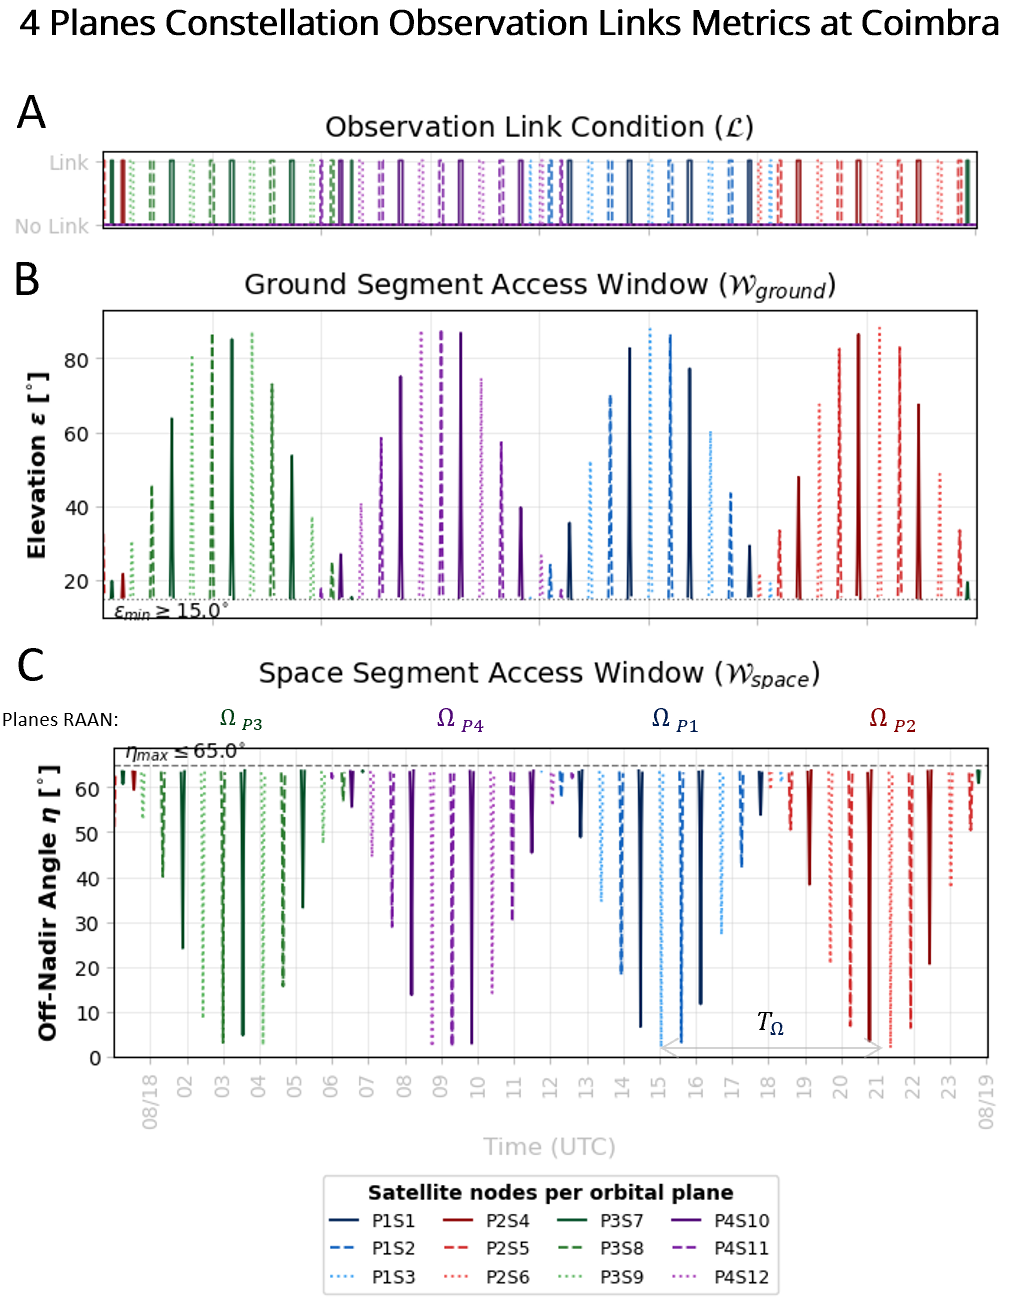
\includegraphics[width=0.95\linewidth]{images/4_planes_Constellation_Observation_Links_at_Coimbra.png}
    \caption{\footnotesize{Observation links at Coimbra for a 4-plane Walker RGTO constellation $\mathcal{C}_{12/4/90}$ derived from $T_{\mathrm{seq,max}} \approx 364.5$\,min.  The inter-plane RAAN spacing is $\delta\Omega = 90^{\circ}$, giving $\Omega_{P1}=100^{\circ}$, $\Omega_{P2}=190^{\circ}$, $\Omega_{P3}=280^{\circ}$, $\Omega_{P4}=10^{\circ}$.  Each plane contributes four high-quality near-nadir passes per day; however, visible gaps between consecutive plane windows indicate insufficient temporal uniformity for the 30-minute monitoring requirement.}}
    \label{fig:obs_links_4planes}
\end{figure}


%%% Zoom Layer η-Sweep Figures (from Chapter~\ref{chapter-9-the-proposed-system-concept})
%%% ================================================================
\section{$\mathcal{C}_{\text{Zoom}}$ Off-Nadir Angle Sweep Maps}
\label{sec:appendix_zoom_eta_sweep}

The following figures complement the baseline ($\eta = 65^{\circ}$) results presented in
Section~\ref{sec:zoom_layer} by showing the temporal-coverage maps for reduced off-nadir
angle configurations ($\eta = 45^{\circ}$, $30^{\circ}$, $15^{\circ}$).

%%% --- Global Temporal Coverage ---
\subsection{Global Domain Temporal Coverage}

\begin{figure}[H]
    \centering
    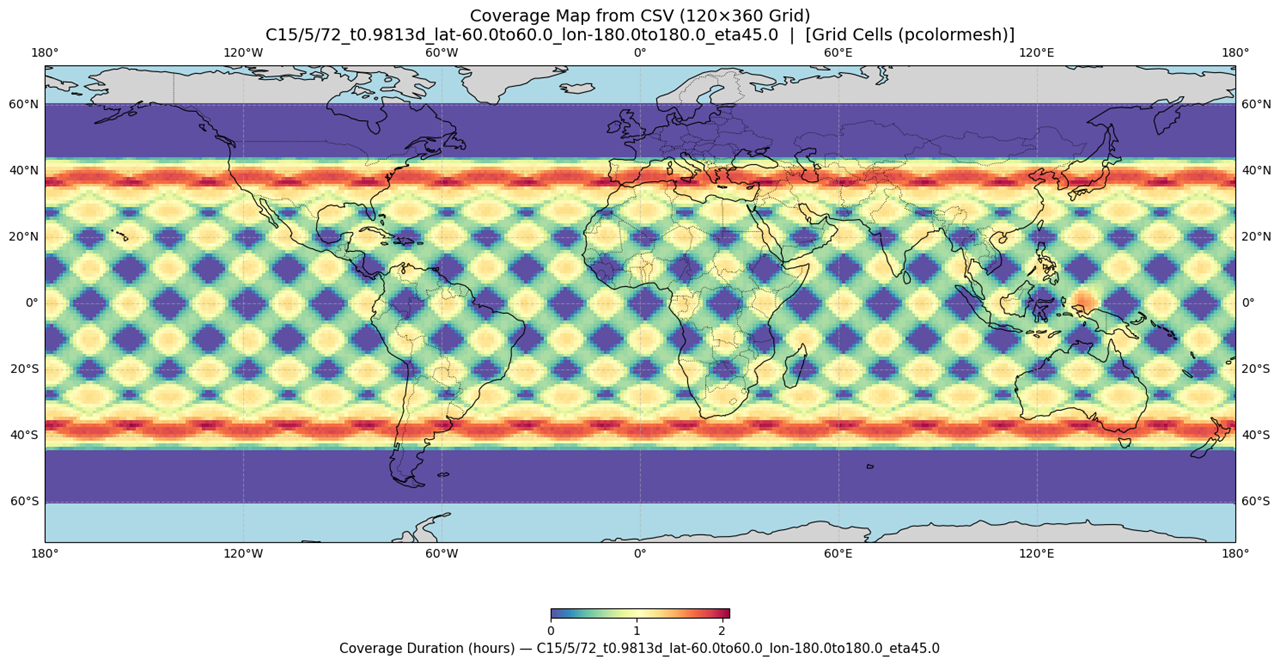
\includegraphics[width=1\linewidth]{images/c_zoom_global_Tcoverage_eta45.png}
    \caption{\footnotesize{Global temporal coverage map for $\eta = 45^{\circ}$.}}
    \label{fig:c_zoom_global_Tcoverage_eta45}
\end{figure}

\begin{figure}[H]
    \centering
    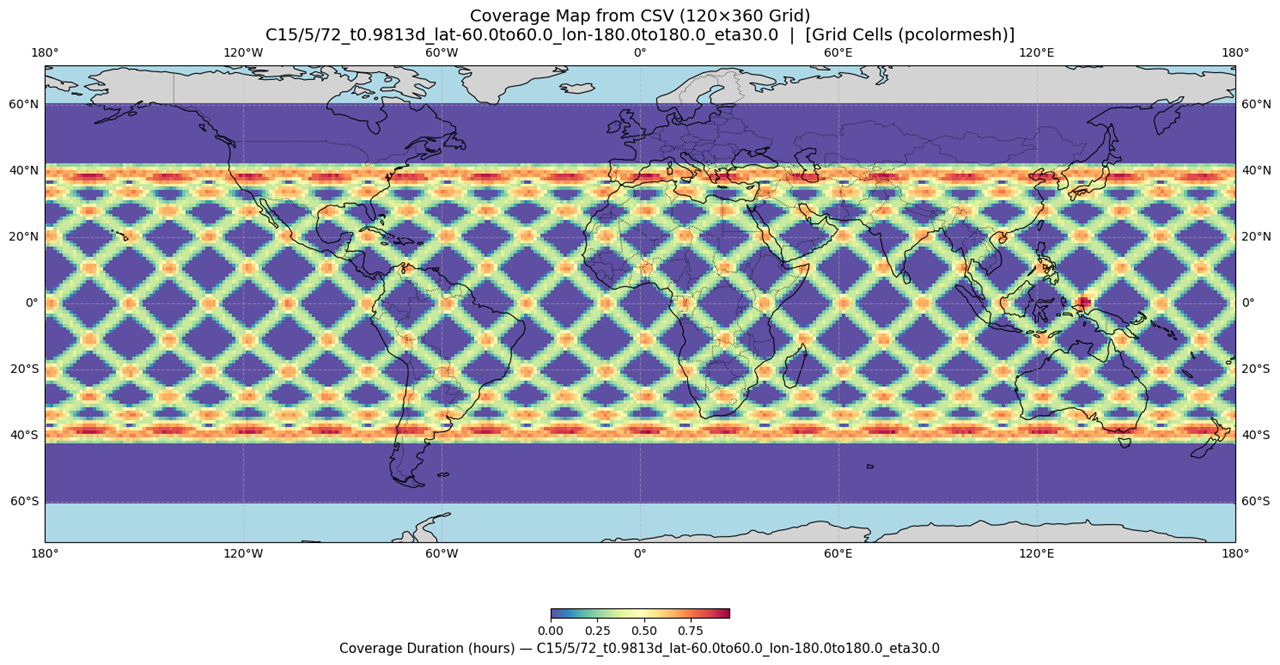
\includegraphics[width=1\linewidth]{images/c_zoom_global_Tcoverage_eta30.png}
    \caption{\footnotesize{Global temporal coverage map for $\eta = 30^{\circ}$.}}
    \label{fig:c_zoom_global_Tcoverage_eta30}
\end{figure}

\begin{figure}[H]
    \centering
    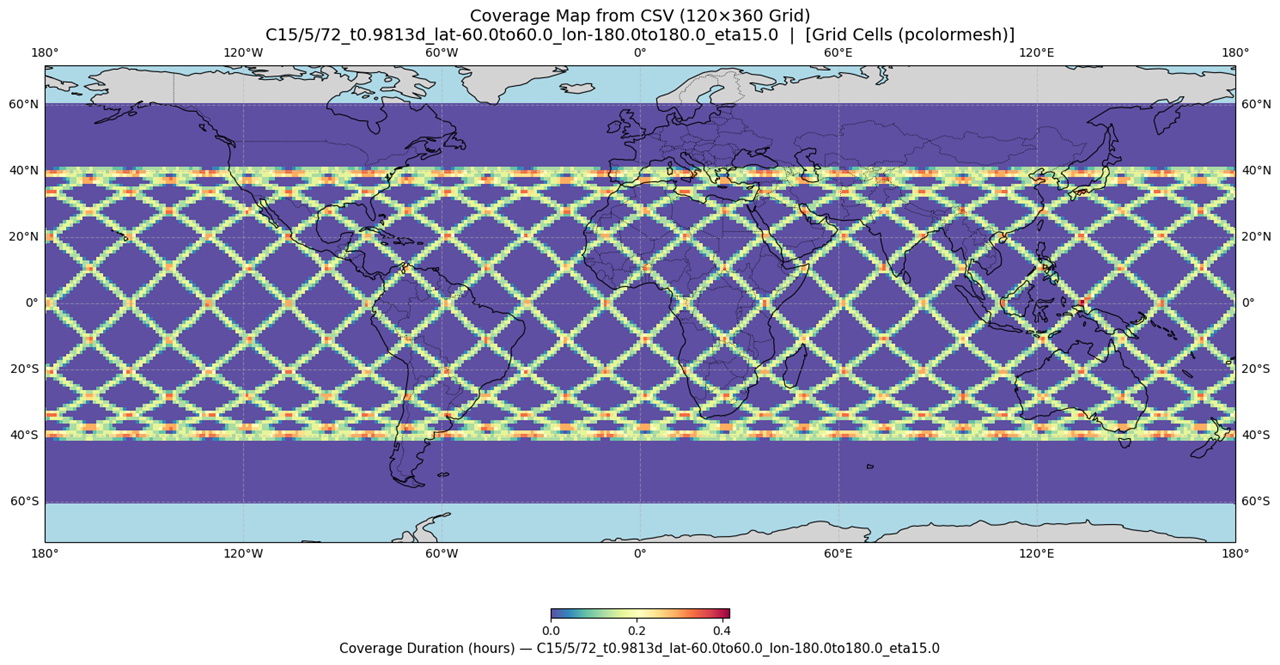
\includegraphics[width=1\linewidth]{images/c_zoom_global_Tcoverage_eta15.png}
    \caption{\footnotesize{Global temporal coverage map for $\eta = 15^{\circ}$.}}
    \label{fig:c_zoom_global_Tcoverage_eta15}
\end{figure}

%%% --- FPR Boundaries ---
\subsection{Fire-Prone Region Boundaries Temporal Coverage}

\begin{figure}[H]
    \centering
    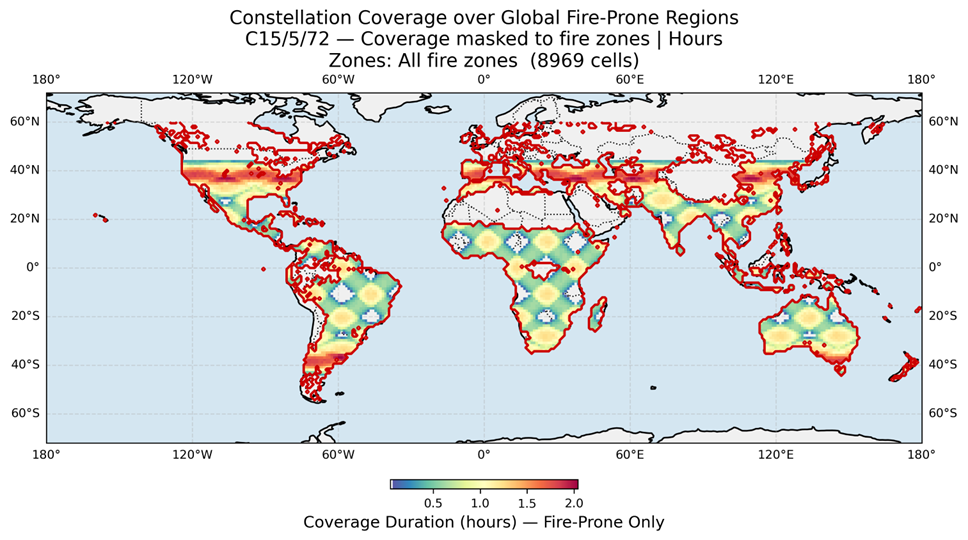
\includegraphics[width=1\linewidth]{images/c_zoom_global_FRP_boundaries_Tcoverage_eta45.png}
    \caption{\footnotesize{FPR boundaries temporal coverage for $\eta = 45^{\circ}$.}}
    \label{fig:c_zoom_global_FRP_boundaries_Tcoverage_eta45}
\end{figure}

\begin{figure}[H]
    \centering
    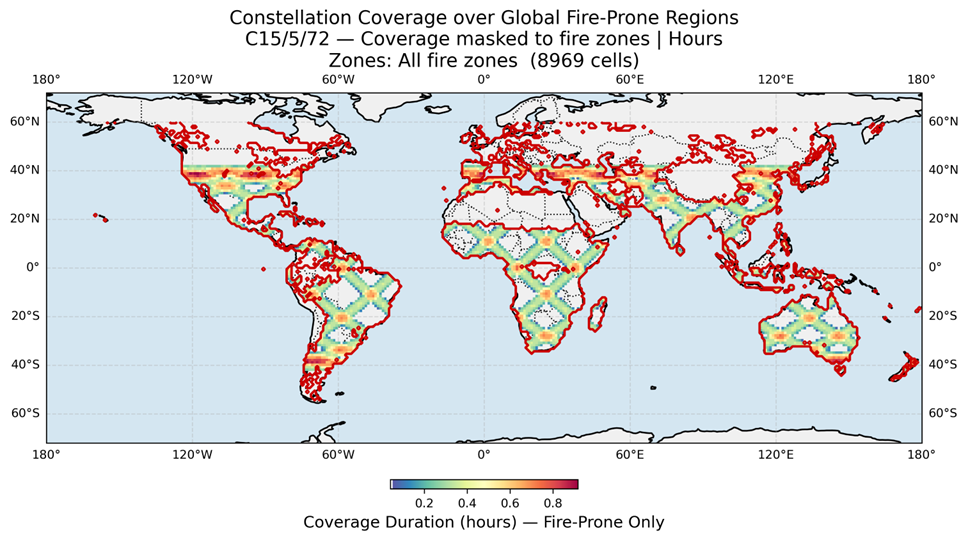
\includegraphics[width=1\linewidth]{images/c_zoom_global_FRP_boundaries_Tcoverage_eta30.png}
    \caption{\footnotesize{FPR boundaries temporal coverage for $\eta = 30^{\circ}$.}}
    \label{fig:c_zoom_global_FRP_boundaries_Tcoverage_eta30}
\end{figure}

\begin{figure}[H]
    \centering
    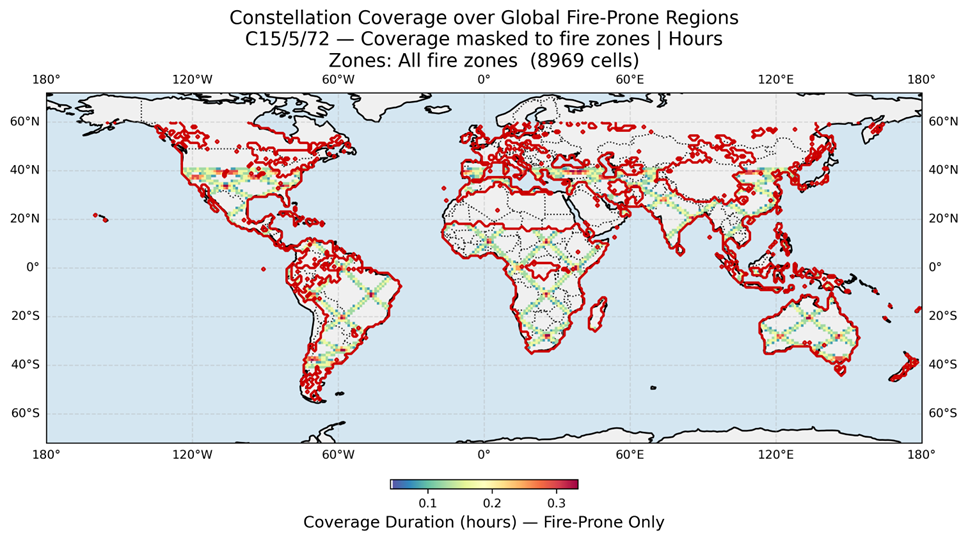
\includegraphics[width=1\linewidth]{images/c_zoom_global_FPR_boundaries_Tcoverage_eta15.png}
    \caption{\footnotesize{FPR boundaries temporal coverage for $\eta = 15^{\circ}$.}}
    \label{fig:c_zoom_global_FPR_boundaries_Tcoverage_eta15}
\end{figure}

%%% --- FPR Recurrent ---
\subsection{Recurrent Fire-Prone Region Temporal Coverage}

\begin{figure}[H]
    \centering
    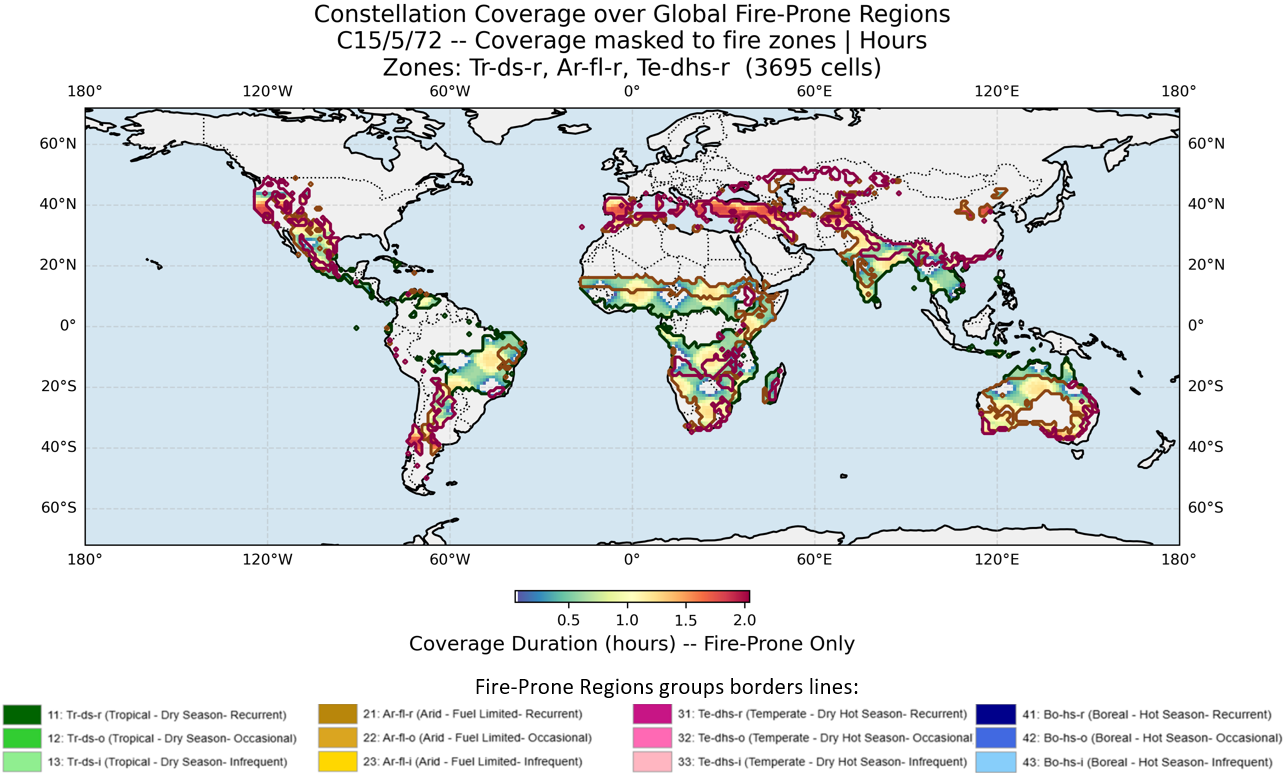
\includegraphics[width=1\linewidth]{images/c_zoom_global_FRP_recurrent_Tcoverage_eta45.png}
    \caption{\footnotesize{Recurrent FPR temporal coverage for $\eta = 45^{\circ}$.}}
    \label{fig:c_zoom_global_FRP_recurrent_Tcoverage_eta45}
\end{figure}

\begin{figure}[H]
    \centering
    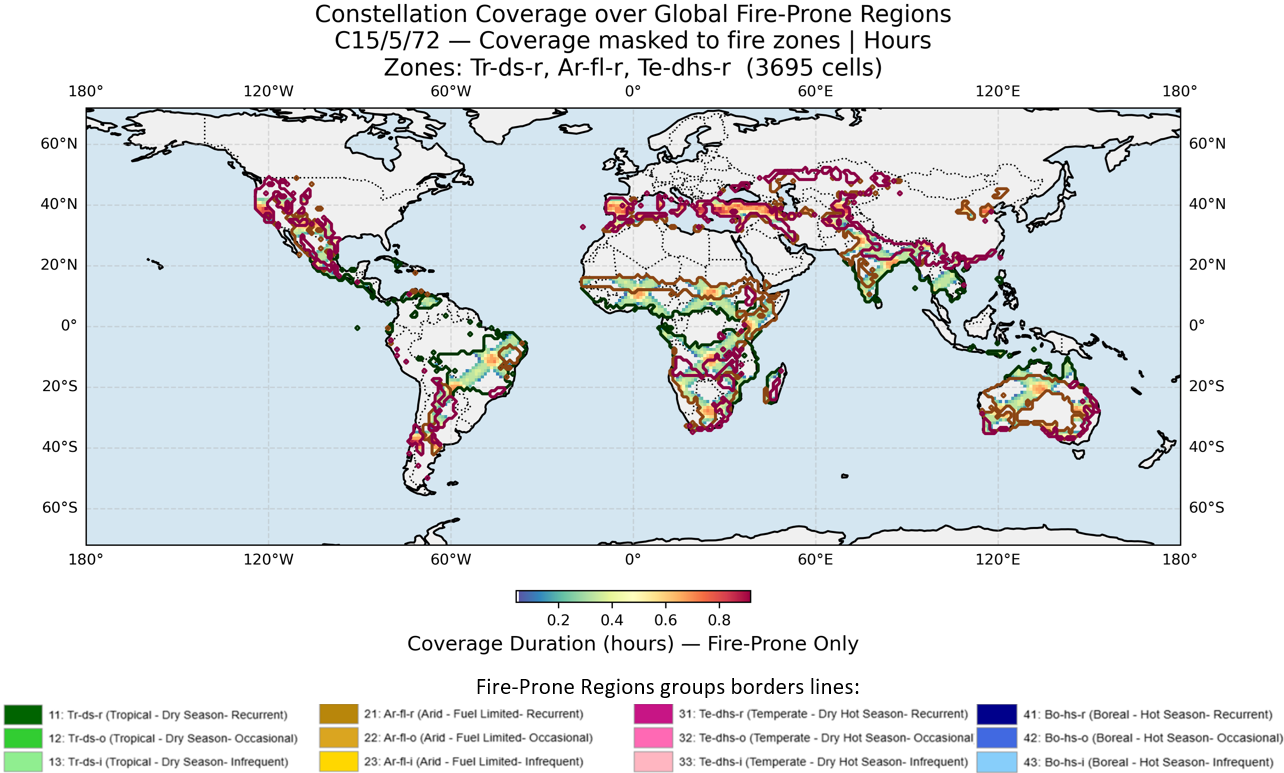
\includegraphics[width=1\linewidth]{images/c_zoom_global_FRP_recurrent_Tcoverage_eta30.png}
    \caption{\footnotesize{Recurrent FPR temporal coverage for $\eta = 30^{\circ}$.}}
    \label{fig:c_zoom_global_FRP_recurrent_Tcoverage_eta30}
\end{figure}

\begin{figure}[H]
    \centering
    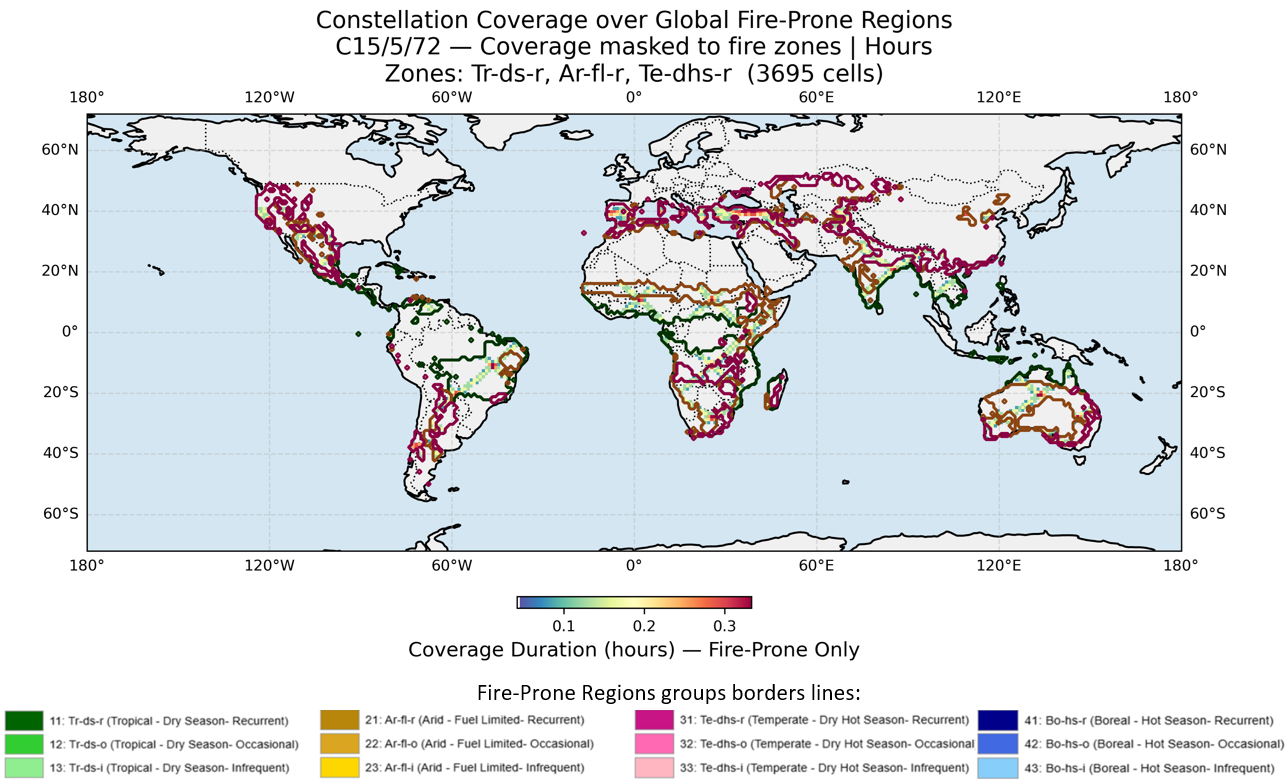
\includegraphics[width=1\linewidth]{images/c_zoom_global_FRP_recurrent_Tcoverage_eta15.png}
    \caption{\footnotesize{Recurrent FPR temporal coverage for $\eta = 15^{\circ}$.}}
    \label{fig:c_zoom_global_FRP_recurrent_Tcoverage_eta15}
\end{figure}

%%% --- FPR Recurrent + Occasional ---
\subsection{Recurrent and Occasional Fire-Prone Region Temporal Coverage}

\begin{figure}[H]
    \centering
    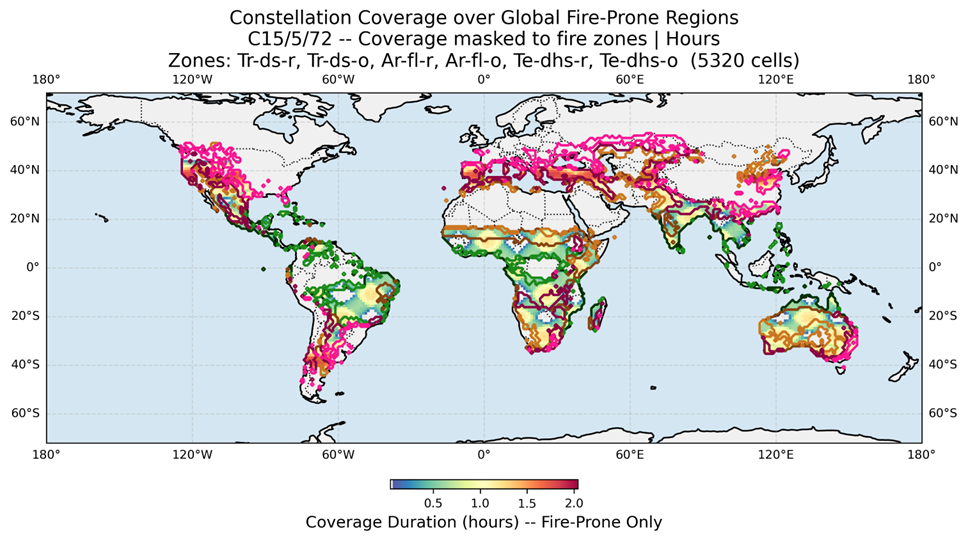
\includegraphics[width=1\linewidth]{images/c_zoom_global_FPR_recurrent_ocasional_Tcoverage_eta45.png}
    \caption{\footnotesize{Recurrent and occasional FPR temporal coverage for $\eta = 45^{\circ}$.}}
    \label{fig:c_zoom_global_FPR_recurrent_ocasional_Tcoverage_eta45}
\end{figure}

\begin{figure}[H]
    \centering
    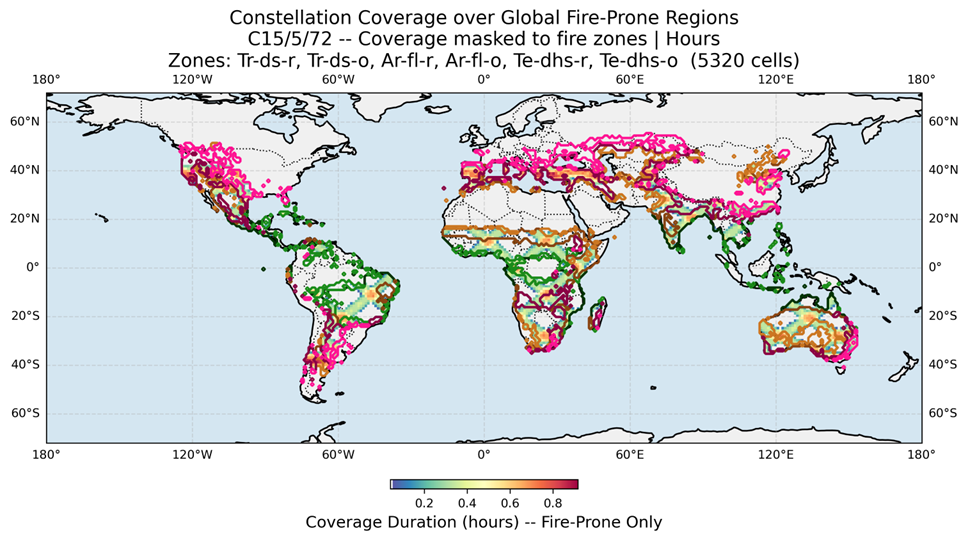
\includegraphics[width=1\linewidth]{images/c_zoom_global_FPR_recurrent_ocasional_Tcoverage_eta30.png}
    \caption{\footnotesize{Recurrent and occasional FPR temporal coverage for $\eta = 30^{\circ}$.}}
    \label{fig:c_zoom_global_FPR_recurrent_ocasional_Tcoverage_eta30}
\end{figure}

\begin{figure}[H]
    \centering
    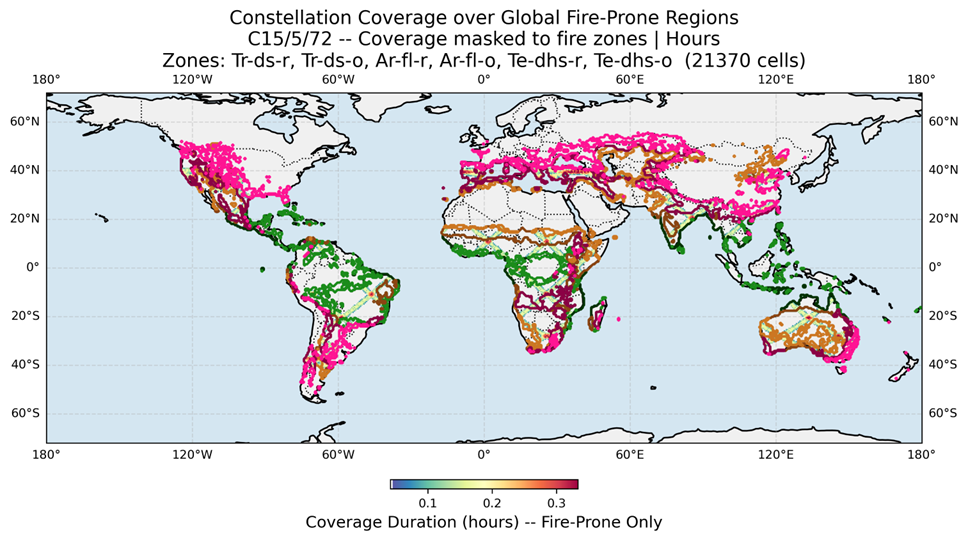
\includegraphics[width=1\linewidth]{images/c_zoom_global_FPR_recurrent_ocasional_Tcoverage_eta15.png}
    \caption{\footnotesize{Recurrent and occasional FPR temporal coverage for $\eta = 15^{\circ}$.}}
    \label{fig:c_zoom_global_FPR_recurrent_ocasional_Tcoverage_eta15}
\end{figure}


%%% ================================================================
%%% FPR Coverage Statistics and Latitude Profile
%%% ================================================================
\section{$\mathcal{C}_{\text{Zoom}}$ FPR Coverage Statistics and Latitude Profile}
\label{sec:appendix_zoom_fpr_statistics}

The following figures provide the detailed bar-chart, scatter-plot, and latitude-profile
breakdowns of the five performance variables across FPR recurrence groups and $\eta$
configurations, complementing the spatial coverage maps in
Section~\ref{sec:global_Domain_fire_prone_regions_statistics}.

\begin{landscape}

%%% --- Normalised ---
\begin{figure}[H]
    \centering
    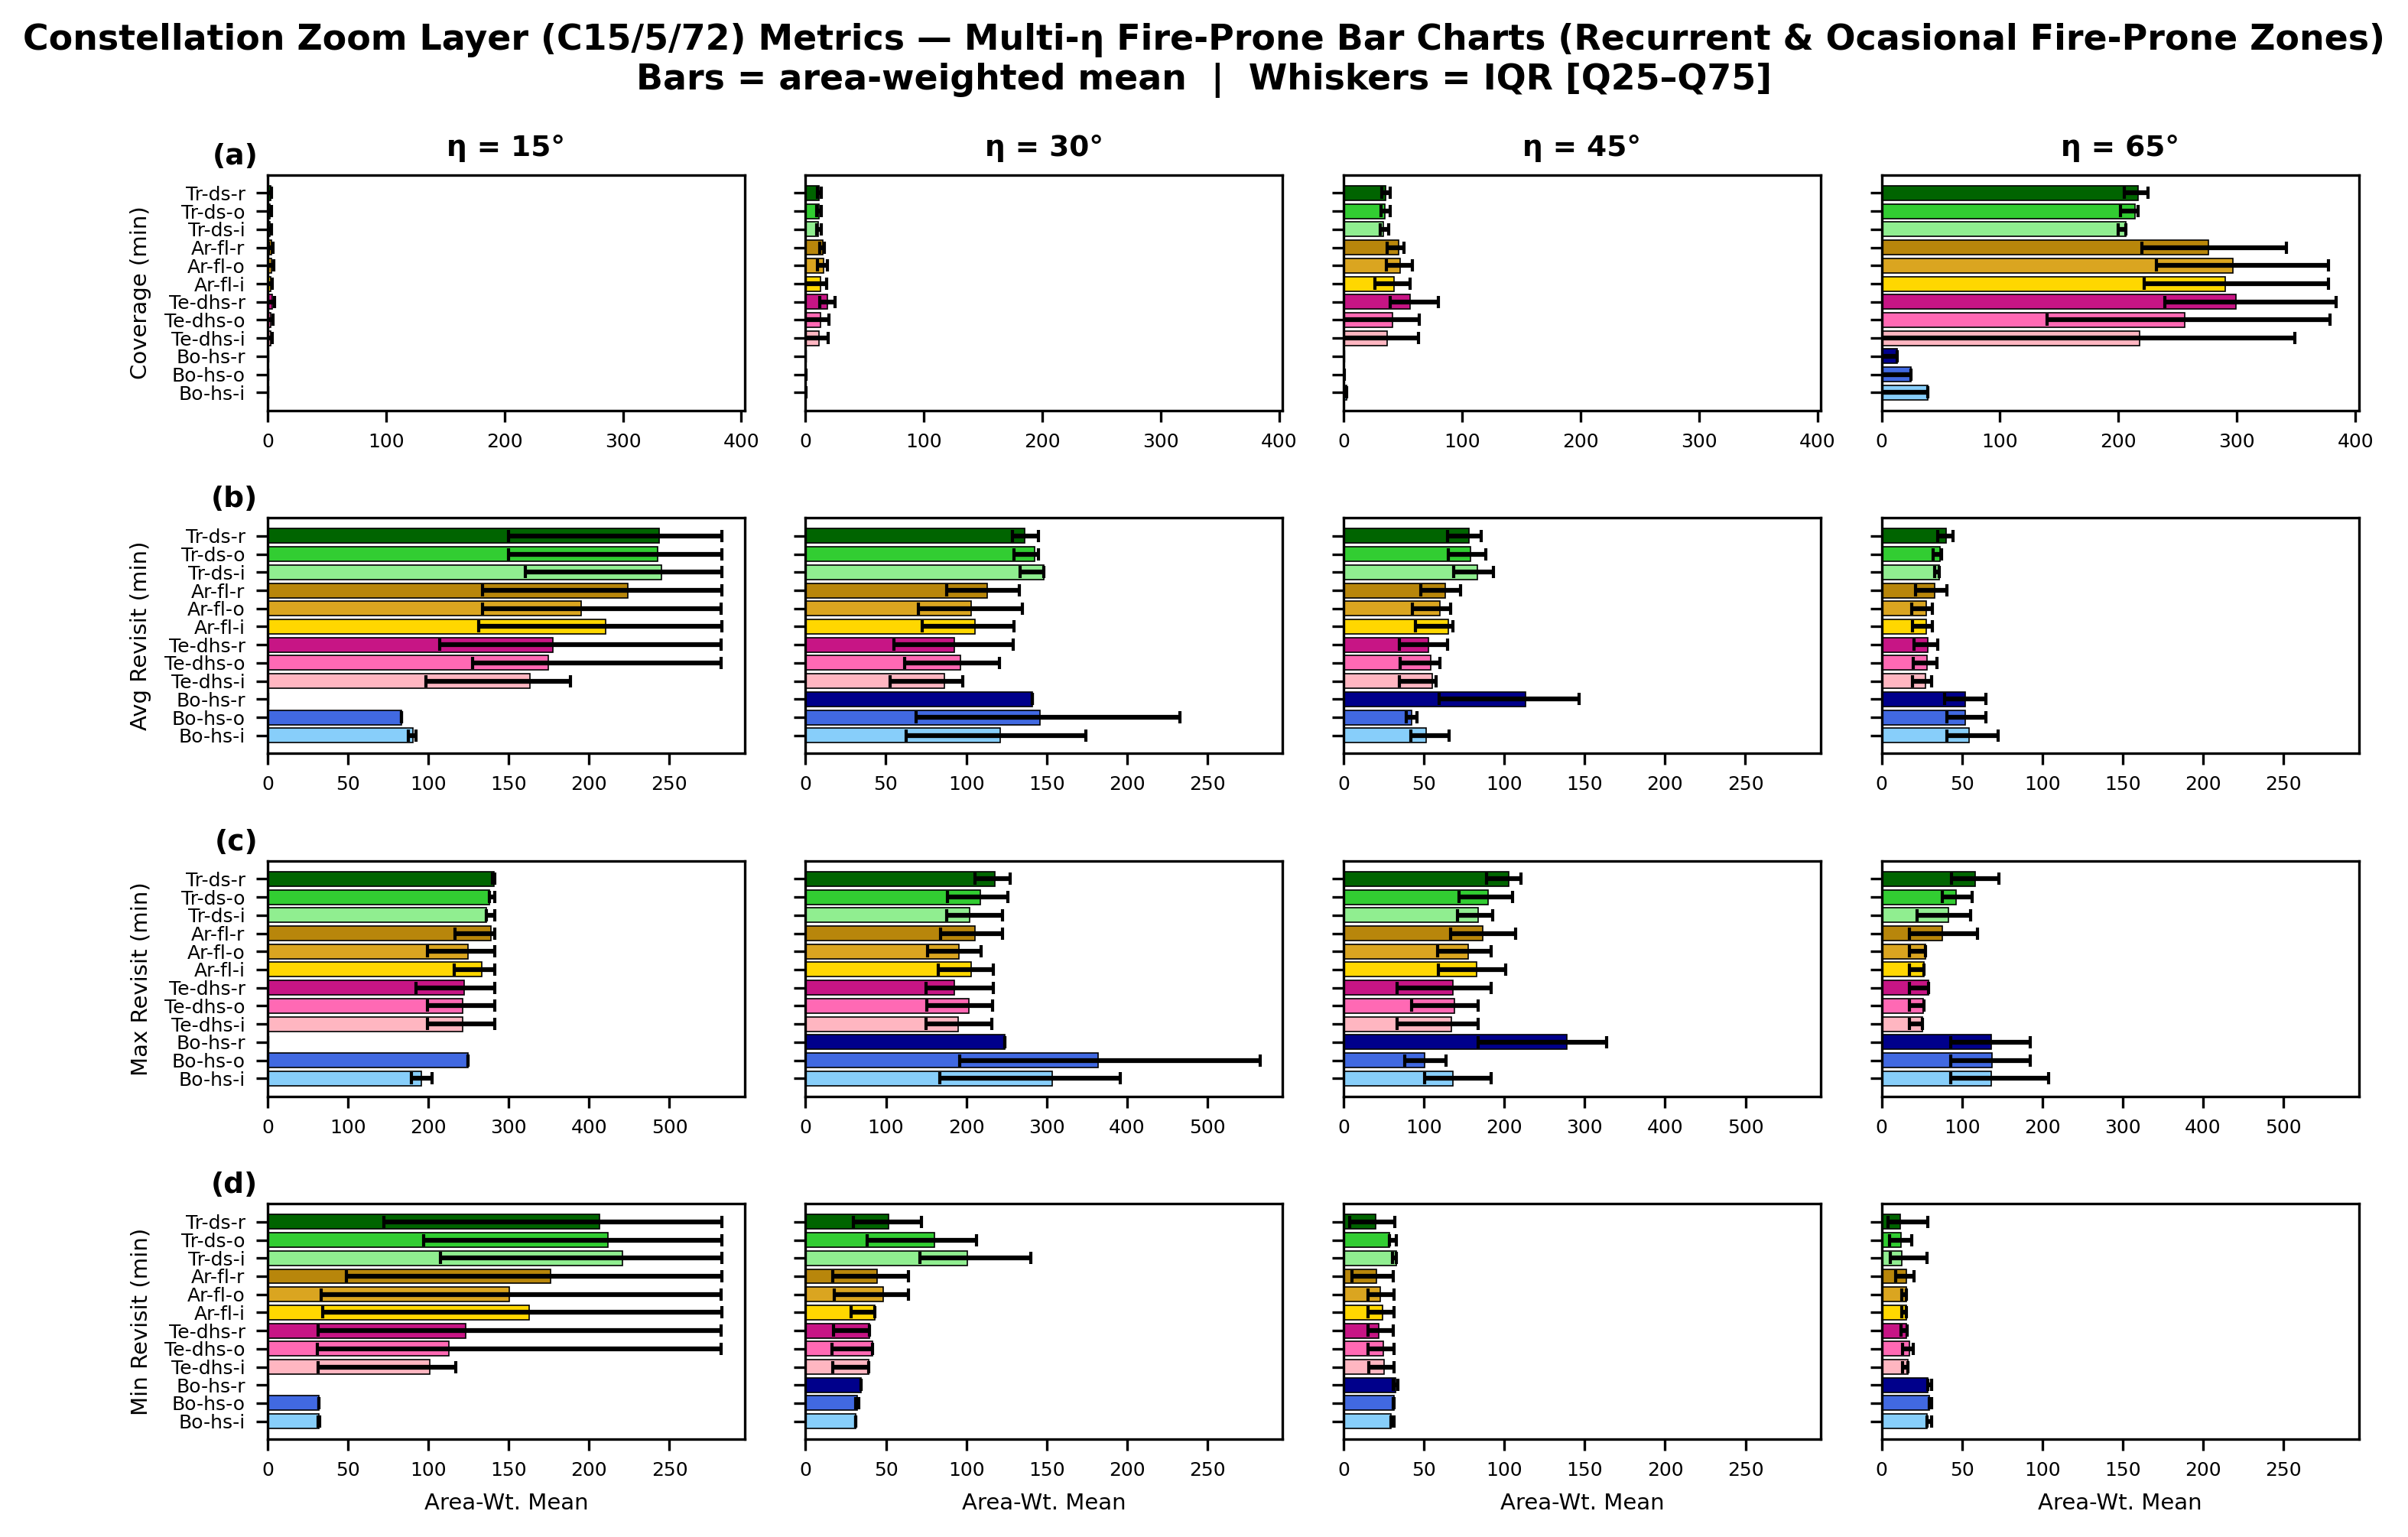
\includegraphics[width=0.85\linewidth,keepaspectratio]{images/c_zoom_metrics_FPR_coverage_statistics_landscape_normalized.png}
    \caption{\footnotesize{Fire-prone region temporal-coverage statistics (normalised) for $\mathcal{C}_{\text{Zoom}}$ across the four $\eta$ configurations ($65^{\circ}$, $45^{\circ}$, $30^{\circ}$, $15^{\circ}$) and the three FPR recurrence groups (recurrent, occasional, infrequent).  Each bar reports the mean $T_{\text{cov}}$ over the masked grid cells; error bars indicate the interquartile range.}}
    \label{fig:c_zoom_metrics_FPR_coverage_statistics}
\end{figure}

\begin{figure}[H]
    \centering
    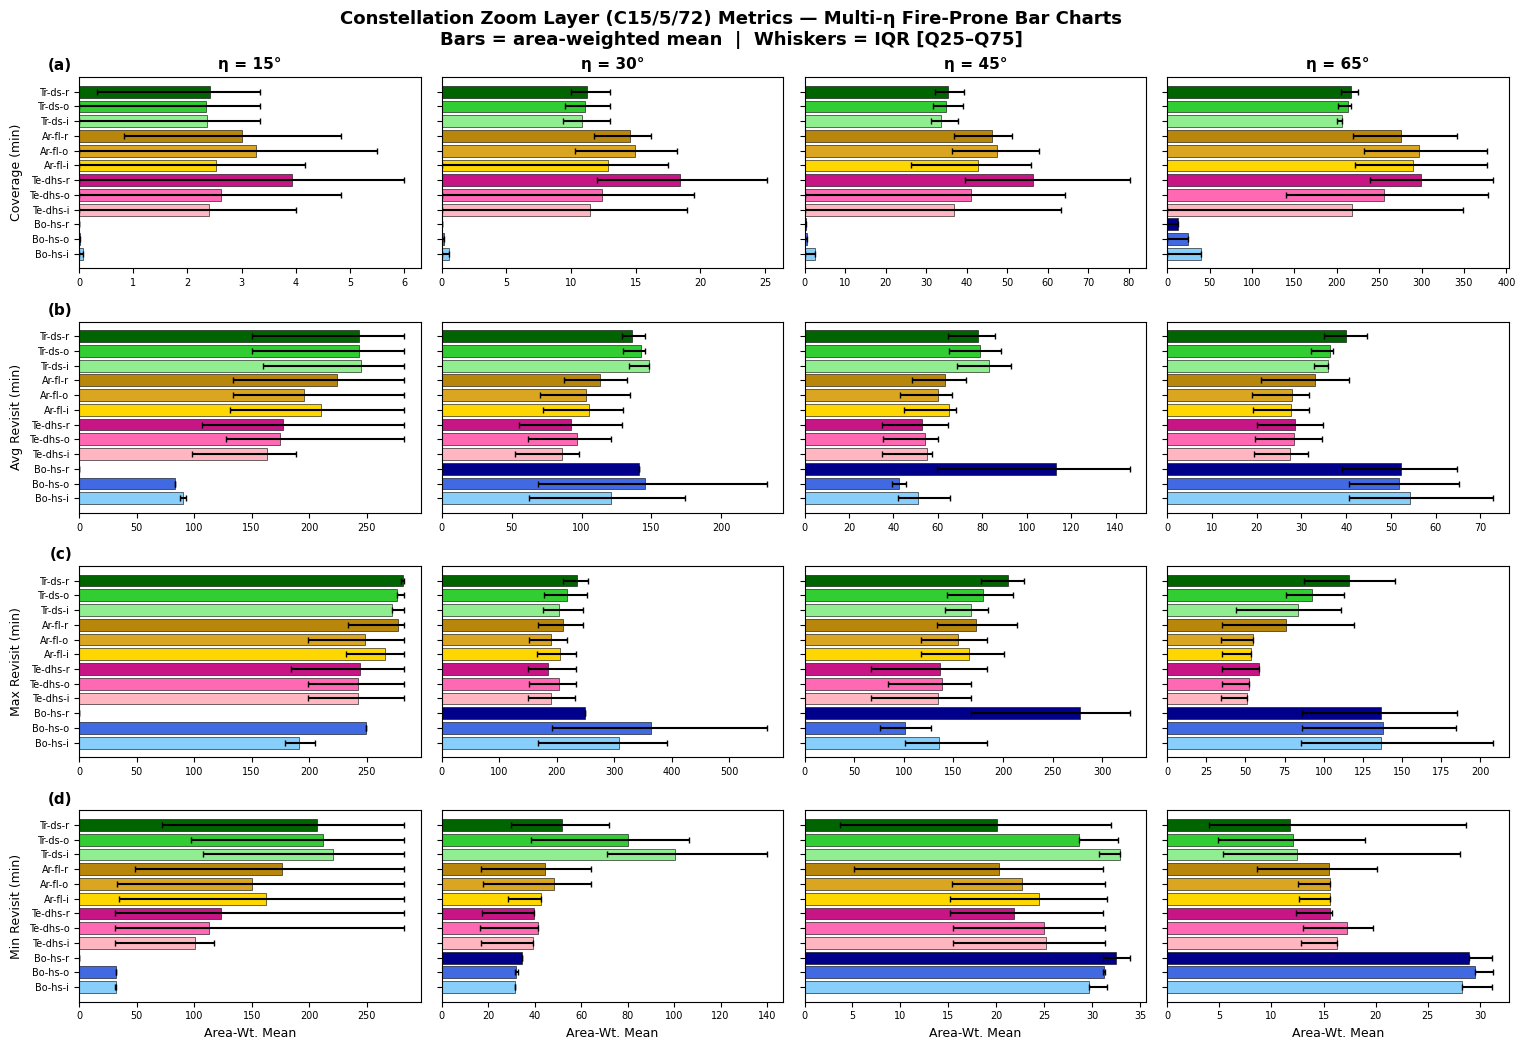
\includegraphics[width=0.85\linewidth,keepaspectratio]{images/c_zoom_metrics_FPR_coverage_statistics_landscape.png}
    \caption{\footnotesize{Fire-prone region temporal-coverage statistics (non-normalised) for $\mathcal{C}_{\text{Zoom}}$ across the four $\eta$ configurations and three FPR recurrence groups.  Absolute $T_{\text{cov}}$ values are shown without per-group normalisation. a) Coverage, b) Average revisit time, c) Max revisit time, d) Min Revisit time}}
    \label{fig:c_zoom_metrics_FPR_coverage_statistics_not_norm}
\end{figure}

\begin{figure}[H]
    \centering
    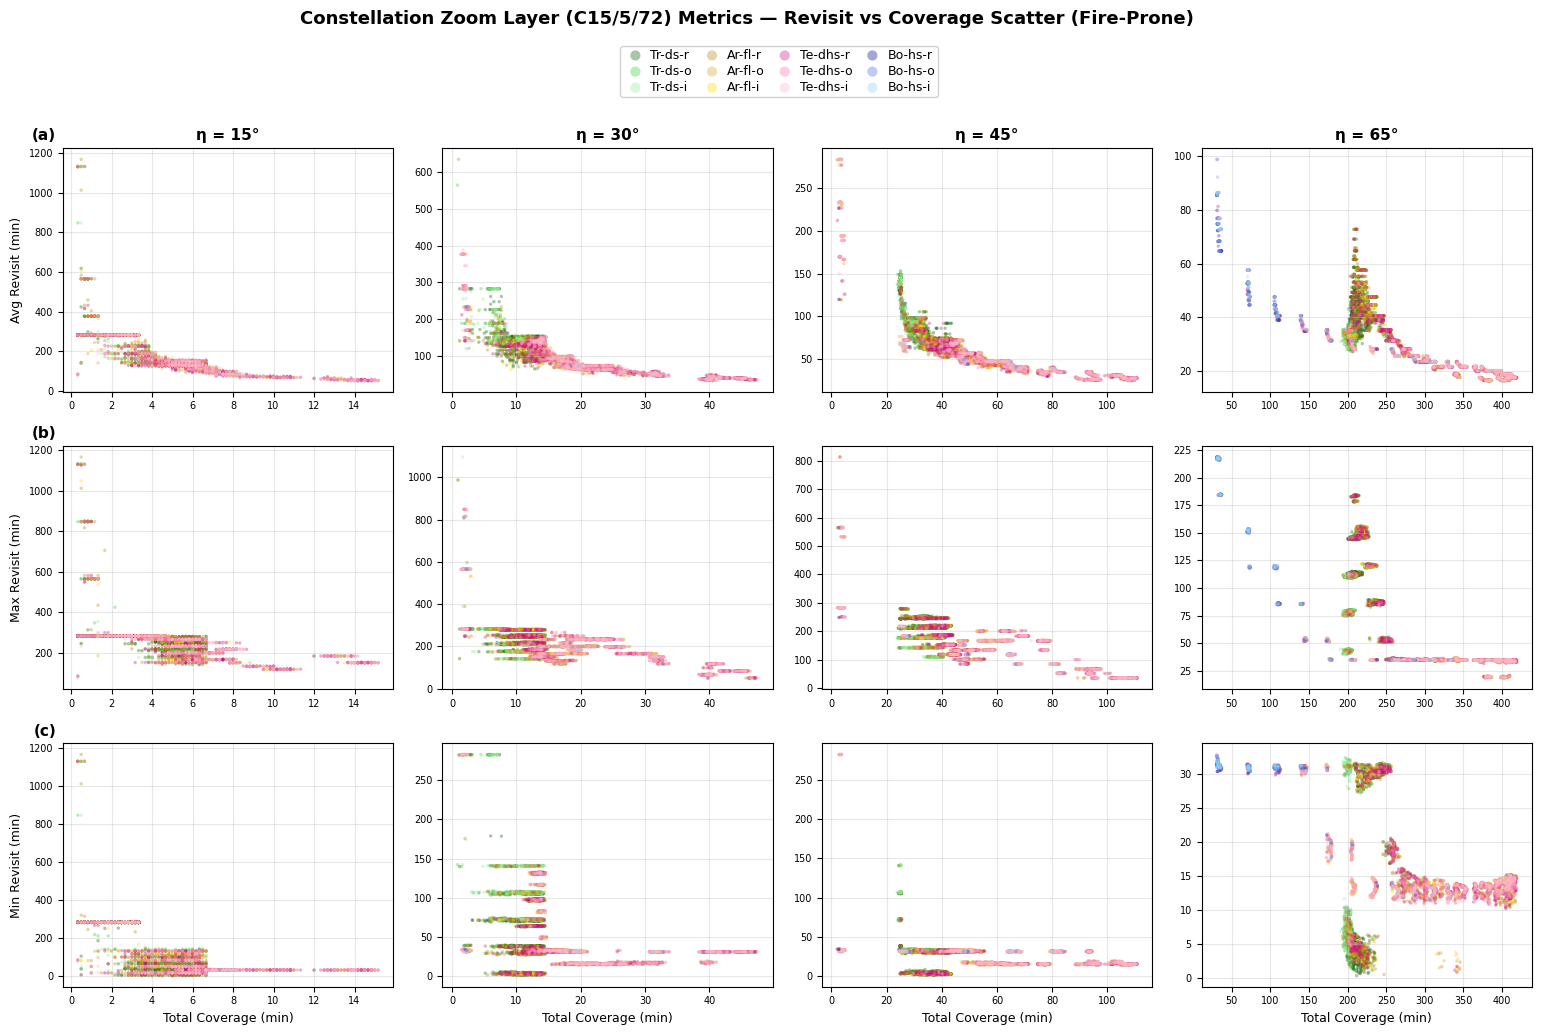
\includegraphics[width=0.85\linewidth,keepaspectratio]{images/c_zoom_metrics_revisitVScoverage_landscape.png}
    \caption{\footnotesize{Revisit time ($\Delta t_{\text{avg}}$) versus temporal coverage ($T_{\text{cov}}$) trade-off for $\mathcal{C}_{\text{Zoom}}$ across FPR recurrence groups and $\eta$ configurations.  Each marker represents one group--$\eta$ combination; wider off-nadir acceptance shifts all groups toward higher coverage and shorter revisit.}}
    \label{fig:c_zoom_metrics_revisitVScoverage}
\end{figure}

\begin{figure}[H]
    \centering
    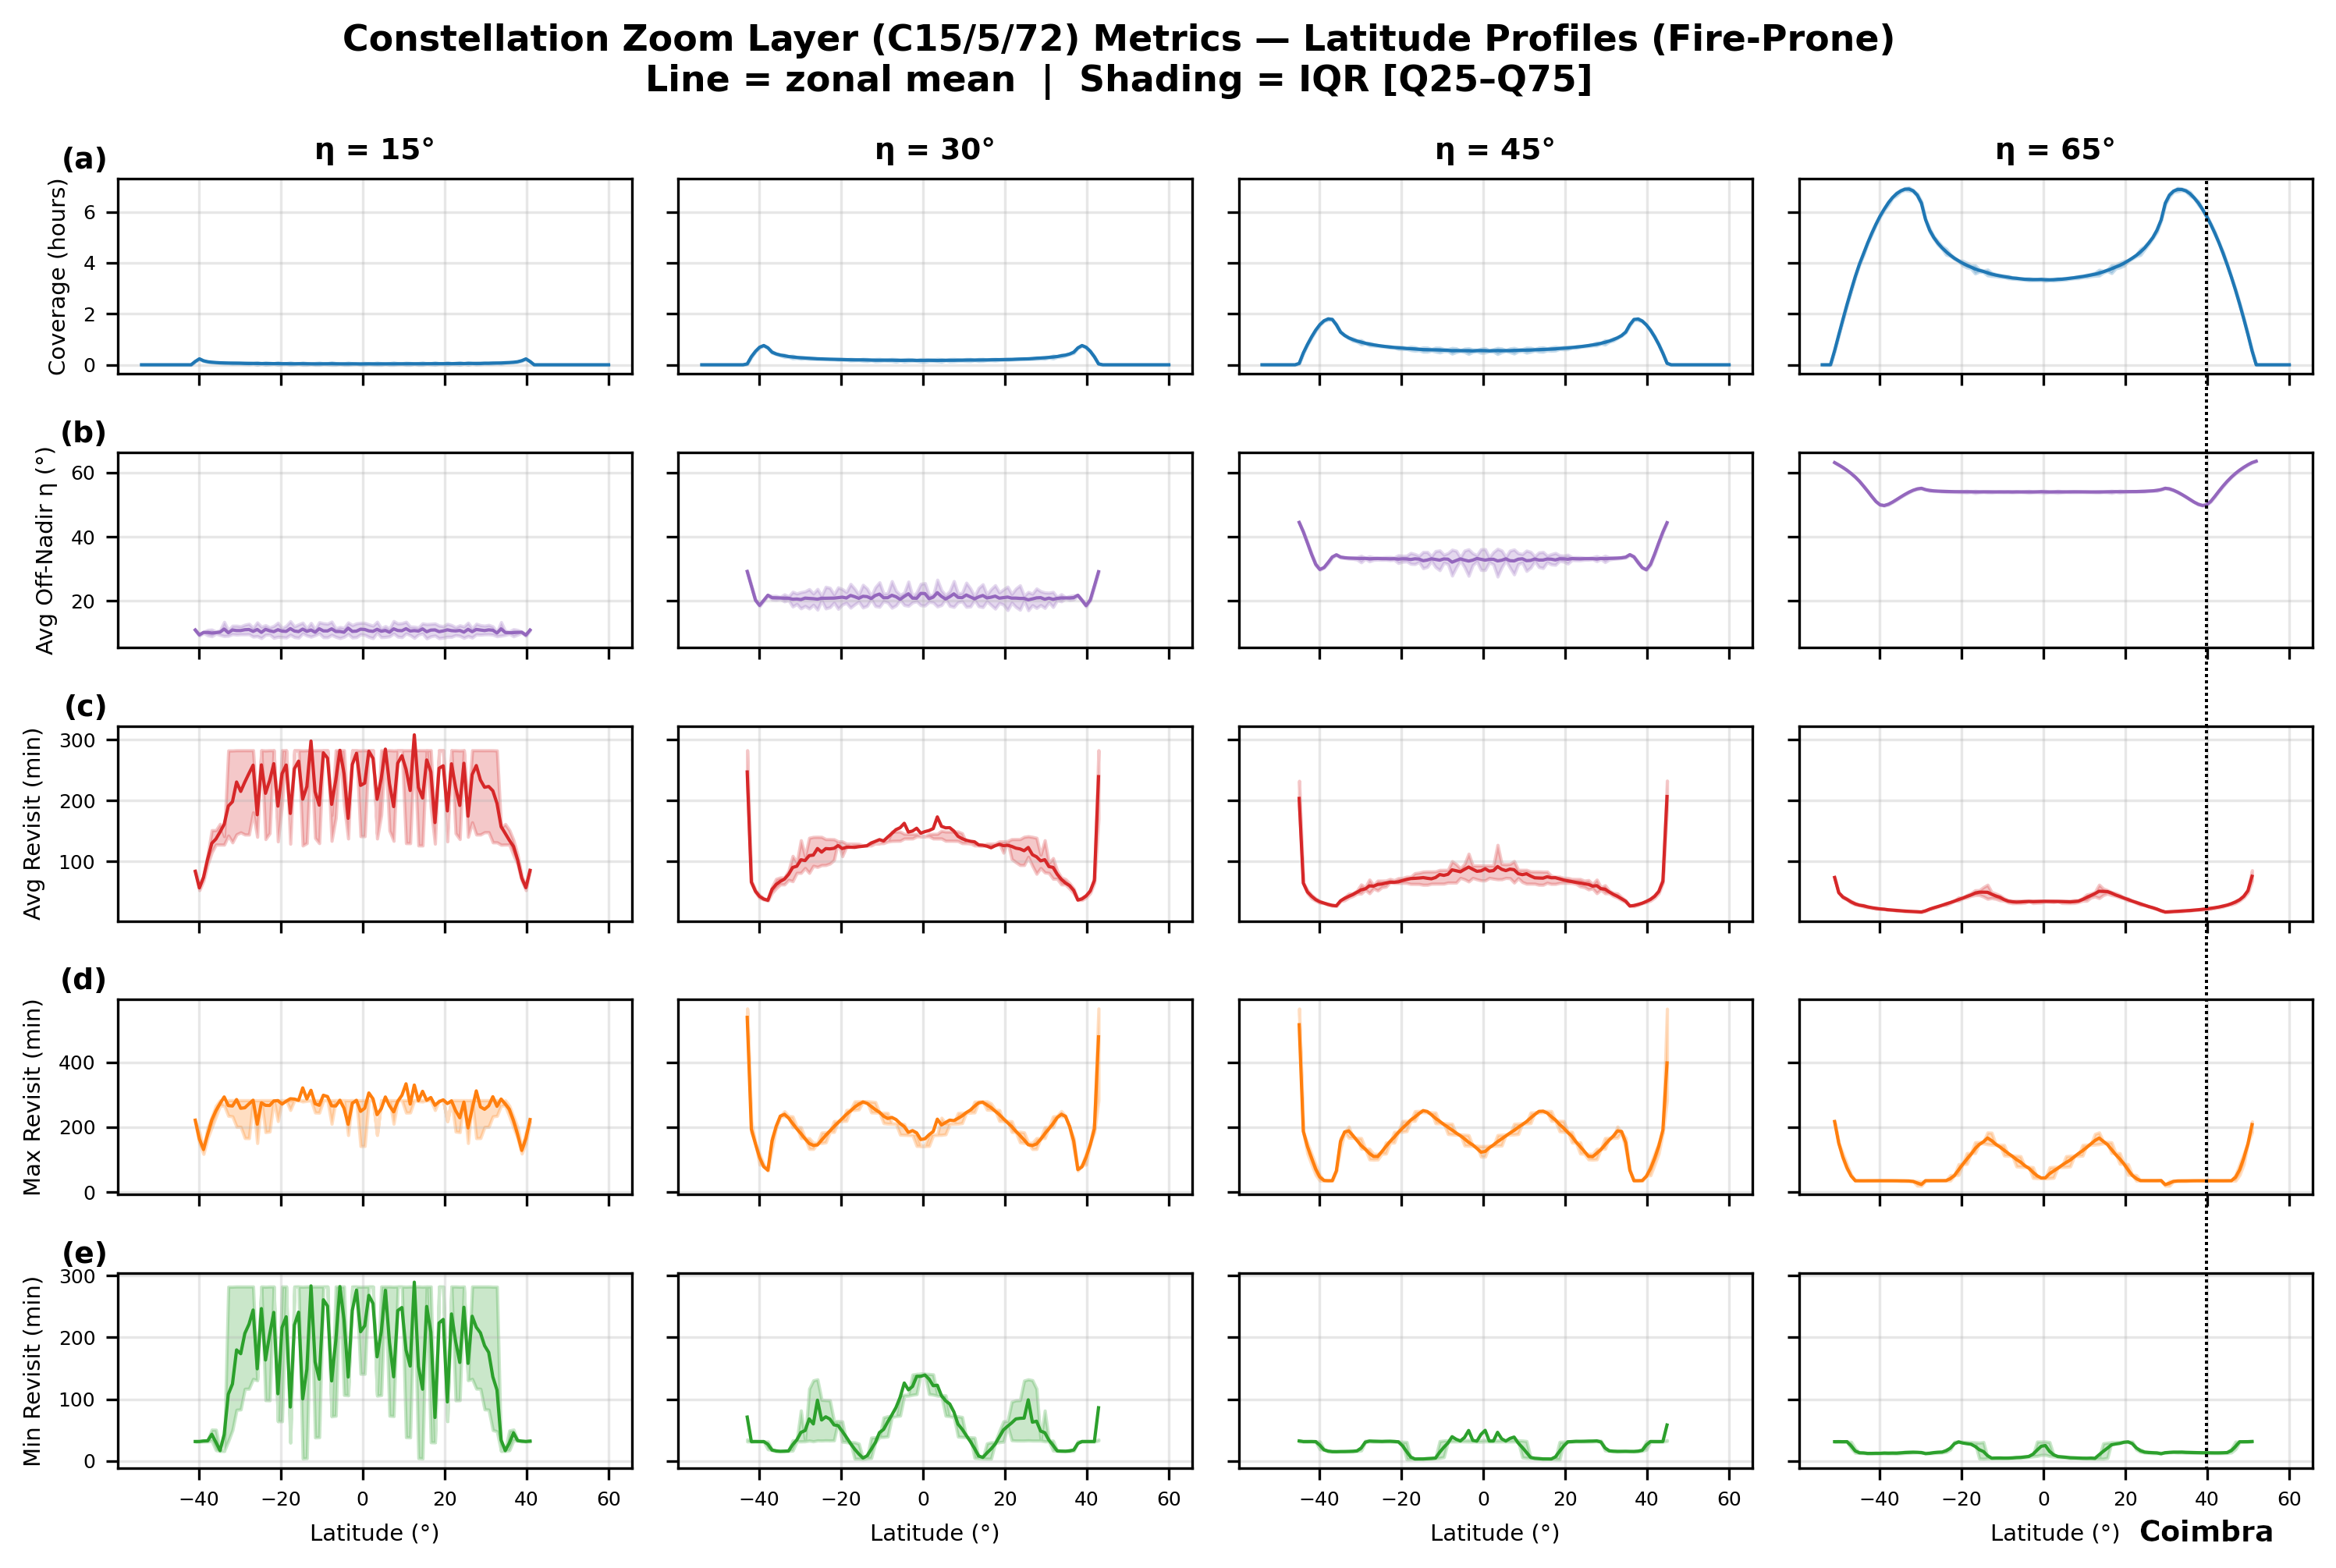
\includegraphics[width=0.85\linewidth,keepaspectratio]{images/c_zoom_metrics_latitude_profile_landscape_normalized.png}
    \caption{\footnotesize{Latitude-dependent temporal-coverage and average-revisit profile (normalised) for $\mathcal{C}_{\text{Zoom}}$ ($\eta = 65^{\circ}$).  Vertical values at $\phi \approx 40^{\circ}$\,N marks the Coimbra core-domain latitude, which falls within the optimal average off-nadir observation angle --- minimum means satellite passes closest to ground nadir axes --- and coverage band. The revisit performance for Portugal is extract from this plot. a) Coverage, b) Average Off-Nadir, c)Average revisit time, d) Max revisit time, e) Min Revisit time}}
    \label{fig:c_zoom_metrics_latitude_profile}
\end{figure}

\begin{figure}[H]
    \centering
    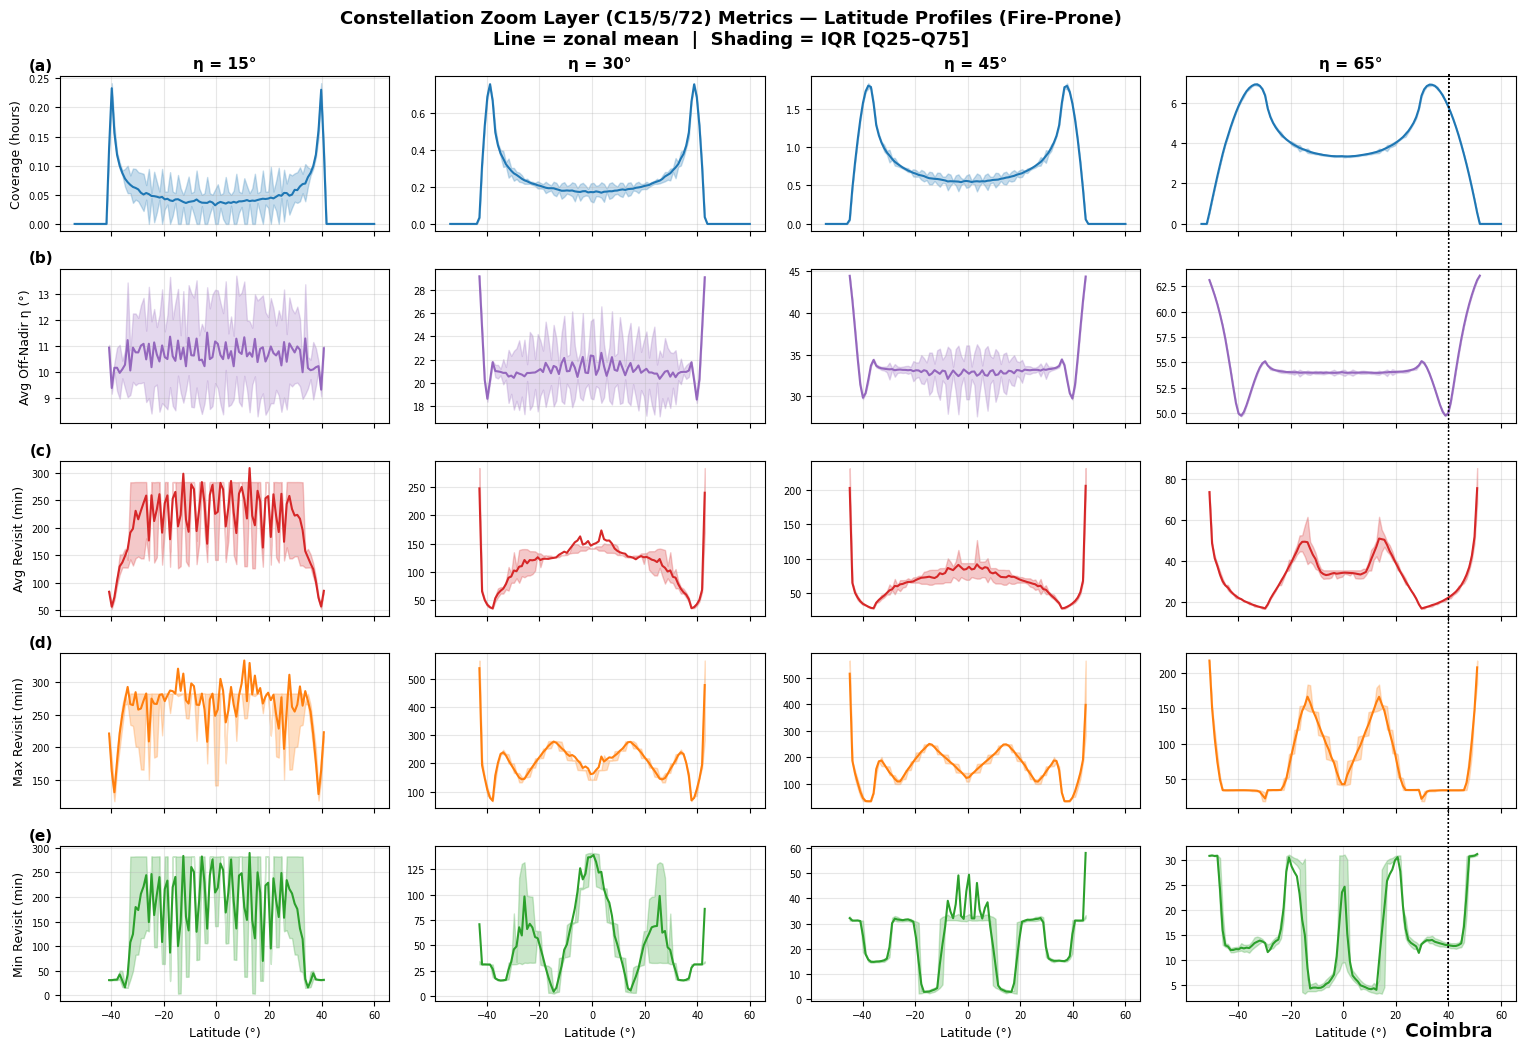
\includegraphics[width=0.85\linewidth,keepaspectratio]{images/c_zoom_metrics_latitude_profile_landscape_not_normalized.png}
    \caption{\footnotesize{Latitude-dependent temporal-coverage and average-revisit profile (non-normalised) for $\mathcal{C}_{\text{Zoom}}$ ($\eta = 65^{\circ}$).Vertical values at $\phi \approx 40^{\circ}$\,N marks the Coimbra core-domain latitude, which falls within the optimal average off-nadir observation angle --- minimum means satellite passes closest to ground nadir axes --- and coverage band. The revisit performance for Portugal is extract from this plot.  Unlike the normalised variant (Fig.~\ref{fig:c_zoom_metrics_latitude_profile}), absolute metric values are plotted on the vertical axes. a) Coverage, b) Average revisit time, c) Max revisit time, d) Min Revisit time.}}
    \label{fig:c_zoom_metrics_latitude_profile_not_norm}
\end{figure}

\end{landscape}